\documentclass[11 pt,a4paper,twoside,openany]{book}
% LTeX: enabled=false

% Idioma y codificación
% \usepackage[utf8]{inputenc}
\usepackage[T1]{fontenc}
\usepackage[spanish,es-tabla]{babel}

% Tipografía y estilos de texto
\usepackage{times}          % Fuente Times New Roman
\usepackage{setspace}       % Ajuste de espaciado entre líneas
\usepackage{textcomp}       % Símbolos adicionales
\usepackage{gensymb}        % Símbolos genéricos (por ejemplo, ° para grados)
\usepackage{enumitem}       % Personalización de listas enumeradas
\usepackage{multicol}
% \usepackage{lipsum} 
\usepackage{comment}        % Para el entorno comment

% Matemáticas
\usepackage{amssymb, amsmath}   % Símbolos y entornos matemáticos
\usepackage{bm}                 % Negritas en matemáticas
% \usepackage{empheq}             % Marcos y resaltado de ecuaciones
% \usepackage{cancel}         % Cancelación de términos en ecuaciones
% \usepackage{siunitx}        % Unidades del SI

% Gráficos y colores
\usepackage{graphicx}               % Inclusión de gráficos
\usepackage{subcaption}             % Subfiguras
\usepackage[table,xcdraw]{xcolor}   % Opciones avanzadas de color
% \usepackage[export]{adjustbox}      % Ajustar alineación de gráficos
% \usepackage{wrapfig}              % Ajustar texto alrededor de imágenes
% \usepackage{pgfplots}             % Graficar funciones directamente 
\usepackage{float}          % Control preciso de la posición de tablas/figuras
% \usepackage{tcolorbox}      % Cajas de texto con formato
\usepackage{pgfgantt}       % Diagramas de Gantt

% Formato y estructura del documento
% \usepackage{vmargin}      % Márgenes personalizados
\usepackage{geometry}       % Márgenes personalizados
\usepackage{fancyhdr}       % Encabezados y pies de página personalizados
\usepackage{tocloft}        % Personalización de la tabla de contenidos
\usepackage{pdflscape}      % Para rotar la página
\usepackage{rotating}       % Permite rotar figuras y tablas

% Citas: ordena y comprime números ([9, 10], [11]–[13])
\usepackage{cite}

% URLs: permite cortarlas en cualquier carácter (evita Underfull \hbox en la bibliografía)
\usepackage{xurl}

% Hipervínculos y navegación
\usepackage[hidelinks]{hyperref}    % Enlaces sin color ni marco visible
\usepackage{bookmark}               % Mejora la navegación en el PDF
\usepackage{titlesec}       % Para redefinir títulos y secciones
\usepackage{etoolbox}       % \patchcmd para el título de la bibliografía

% Tablas avanzadas
\usepackage{array}          % Mejoras en tablas
\usepackage{multirow}       % Combinar filas en tablas
\usepackage{tabularray}     % Alternativa moderna a tabular
\UseTblrLibrary{booktabs}
\SetTblrDefault{conthead = {}}

% Diagramas
\usepackage{tikz}
\usetikzlibrary{positioning,arrows.meta,calc,decorations.pathreplacing}

% LTeX: enabled=false

% Margenes
\geometry{
  a4paper,
  inner=2.5cm,
  outer=2cm,
  top=4cm,
  bottom=2.3cm,
  headheight=2cm,
  headsep=0.5cm,
  footskip=1cm
}

% Espaciado general del texto
% \spacing{1.5}
\setstretch{1.5}

% No estirar espacios verticales para igualar el final de cada página
% (book con twoside usa \flushbottom por defecto → Underfull \vbox)
\raggedbottom

% Eliminar espaciado de enumerate e itemize
\setlist[enumerate,itemize]{itemsep=0pt, topsep=0pt}

% Para que todos los Figura xx aparezcan en negrita
\captionsetup[figure]{labelfont=bf}

% Para que todos los Tabla xx aparezcan en negrita
\DefTblrTemplate{caption-tag}{default}{\bfseries Tabla\hspace{0.25em}\thetable}
\DefTblrTemplate{caption-sep}{default}{\bfseries :\enskip}

% Estilo para páginas de título (como \maketitle)
\fancypagestyle{plain}{
    \fancyhf{}
    \renewcommand{\headrulewidth}{1 pt}
    \renewcommand{\footrulewidth}{1 pt}
    \fancyhead[RO,LE]{Aranda Brian Ezequiel, Wlodeck Fabricio Joaquin}
    \fancyfoot[LE,RO]{\textbf{Pág. N° \thepage}}
}

% Estilo general para el documento
\pagestyle{fancy}
    \fancyhf{}
    \renewcommand{\headrulewidth}{1 pt}
    \renewcommand{\footrulewidth}{1 pt}
    % Encabezado: Siempre a la derecha (R) en todas las páginas
    \fancyhead[LE]{\textbf{\leftmark}}
    \fancyhead[RO]{\textbf{\rightmark}}
    % Pie de página: Número alternado (izquierda en pares, derecha en impares)
    \fancyfoot[LE,RO]{\textbf{Pág. N° \thepage}} 

% Texto parte de las longtable (tablas de varias páginas)
\DefTblrTemplate{contfoot-text}{default}{Continua en la siguiente página $\cdots$}
\DefTblrTemplate{conthead-text}{default}{(Continuación)}

% Definición del espaciado de indice
\setlength{\cftbeforetoctitleskip}{-10 pt}       % Espacio antes de indice general
\setlength{\cftaftertoctitleskip}{5 pt}         % Espacio despues de indice general

% Idem que lo anterior pero para el indice de figuras y tablas
\setlength{\cftbeforeloftitleskip}{-10 pt}       
\setlength{\cftafterloftitleskip}{20 pt}         
\setlength{\cftbeforelottitleskip}{-10 pt}       
\setlength{\cftafterlottitleskip}{20 pt}       

% Cambiar el tamaño de la palabra "Índice"
\renewcommand{\cfttoctitlefont}{\Huge\bfseries} % Tamaño Huge y negrita

% Usar el punto como separador decimal
\decimalpoint

% Configuración de la Bibliografía
\renewcommand{\bibname}{Bibliografía}
\patchcmd{\thebibliography}
  {\chapter*{\bibname}}
  {\chapter{\bibname}\footnotesize}
  {}{}

\begin{comment}
    \titleformat{nombre de la parte a modificar}
        {Formato de la sección}    
        {Número y separador}                             
        {Separación entre numero y tituli}                  
        {Código adicional}
        [Otra configuración, por ejemplo línea]
\end{comment}

% Redefinición del formato de \chapter
\titleformat{\chapter}[hang]
    {\normalfont\huge\bfseries} % sin \centering → alineado a la izquierda
    {}              
    {0 cm}
    {\MakeUppercase}
    \titlespacing*{\chapter}{0 pt}{-30 pt}{5 pt} % {izq}{antes}{después}
    \setcounter{secnumdepth}{-1}
    \setlength{\cftbeforechapskip}{15 pt}

% Redefinición del formato de \section
\titleformat{\section}[block]
    {\normalfont\LARGE\bfseries}    
    {}                    
    {0 cm}                         
    {}                
    %[\vspace{0.5ex}\titlerule] 
    \titlespacing*{\section}{0pt}{0.3 cm}{*1}

% Redefinición del formato de \subsection
\titleformat{\subsection}
    {\normalfont\large\bfseries}    % Formato de la subsección
    {}                              % Elimina el número
    {0 pt}                          % Sangría
    {}                              % Código adicional (opcional)
    \titlespacing*{\subsection}{0pt}{0.2 cm}{*1}

% Redefinición del formato de \subsubsection
\titleformat{\subsubsection}
    {\normalfont\normalsize\bfseries}   % Formato de la subsubsección
    {}                                  % Elimina el número
    {0 pt}                              % Sangría
    {}                                  % Código adicional (opcional)
    \titlespacing*{\subsubsection}{0pt}{0.2 cm}{*1}

% Elimina la numeración del indice
    
    % Secciones
    \renewcommand{\cftsecpresnum}{}         % Elimina el prefijo de numeración
    \renewcommand{\cftsecaftersnum}{}       % Elimina el sufijo de numeración
    \renewcommand{\cftsecnumwidth}{0 pt}    % Ancho de la numeración (0pt para eliminarla)
    \renewcommand{\thesection}{}            % Elimina el número de sección en el índice
    
    % Subsecciones
    \renewcommand{\cftsubsecpresnum}{}          % Elimina el prefijo de numeración
    \renewcommand{\cftsubsecaftersnum}{}        % Elimina el sufijo de numeración
    \renewcommand{\cftsubsecnumwidth}{0 pt}     % Ancho de la numeración (0pt para eliminarla)
    \renewcommand{\thesubsection}{}             % Elimina el número de subsección en el índice
    
    % Subsubsecciones
    \renewcommand{\cftsubsubsecpresnum}{}       % Elimina el prefijo de numeración
    \renewcommand{\cftsubsubsecaftersnum}{}     % Elimina el sufijo de numeración
    \renewcommand{\cftsubsubsecnumwidth}{0 pt}  % Ancho de la numeración (0pt para eliminarla)
    \renewcommand{\thesubsubsection}{}          % Elimina el número de subsubsección en el índice
\begin{document}

    % Titulo
    % LTeX: enabled=false

\begin{titlepage} \centering

    % Logo y nombre de la facultad
    \begin{minipage}{0.6\textwidth}
        \begin{flushright}
            \LARGE \textbf{Universidad Nacional de Misiones} \par 
            \Large \textbf{Facultad de Ingeniería}
        \end{flushright}
    \end{minipage}
    \hspace{0.5 cm}
    \begin{minipage}{0.3\textwidth}
         
\includegraphics[width = 4 cm , height = 1.75 cm]{img/Logo_UNaM.png}
    \end{minipage}

    % Titulo
    \vspace{1 cm}
    \huge \textbf{Trabajo Práctico N.º 3}
    \par \vspace{-0.75 cm}
    \rule{\linewidth}{0.7 mm}

        \par \vspace{-0.5 cm}
        \Huge \textbf{KERALYTIX}

        \par \vspace{0.25 cm}
        
\includegraphics[width = 3 cm, height = 3 cm]{img/logotipo_solo.png}

        \large Sistema de soporte para la decisión clínica temprana del queratocono mediante IA multimodal

    \rule{\linewidth}{0.7 mm}

    % Grupo
    % \par \vspace{-1 cm}
    \textbf{\Large Grupo N.º 7}
    \vspace{0.2 cm}

    % Autores, Tutor y Docentes
    \begin{flushleft}
        \Large \textbf{Autores:} \par
        \Large \hspace{0.5 cm} Aranda, Brian Ezequiel \par
        \Large \hspace{0.5 cm} Wlodeck, Fabricio Joaquín  \par
        
        \vspace{0.25 cm}
        \Large \textbf{Docente tutor:} \par
        \Large \hspace{0.5 cm} Ing. Krujoski, Matías Gabriel\par
        
        \vspace{0.25 cm}
        \Large \textbf{Docentes de la cátedra:} \par
        \Large \hspace{0.5 cm} Dr. Ing. Javier Kolodziej \par
        \Large \hspace{0.5 cm} Dra. Ing. Romina Niezwida 
    \end{flushleft}
    \vspace{1.5 cm}

    % Fecha
    {\Large \textbf{Oberá, Misiones - 30 de octubre de 2026}} \par
    \Large \textbf{Cátedra: Proyecto final integrador [IC-522]} 
    
\end{titlepage}

    % Resumen y palabras clave
    \newpage
\thispagestyle{empty}

\begin{center}
    \Large \textbf{RESUMEN}
\end{center}

    Este proyecto propone el desarrollo de KERALYTIX, un sistema de soporte a la decisión clínica para oftalmólogos, basado en inteligencia artificial multimodal, que asiste en la detección temprana del queratocono. KERALYTIX procesa de forma automatizada mapas corneales obtenidos con equipos de topografía y tomografía, combinándolos con datos clínicos estructurados del paciente para generar una predicción diagnóstica fundamentada en la evidencia clínica. El prototipo se desarrolla sobre un conjunto de datos público de estudios Orbscan\textsuperscript{\scriptsize\textregistered}{} y se ofrece como una aplicación web bajo un modelo de suscripción.

    KERALYTIX se enmarca como un Software como Producto Médico (SaMD\footnote{Por sus siglas en inglés, \textit{Software as a Medical Device}.}) que integra redes neuronales convolucionales para el análisis de imágenes, una rama de procesamiento de datos clínicos estructurados y un mecanismo de fusión multimodal que permite capturar patrones que serían imperceptibles al analizar cada modalidad por separado. Además, incorpora herramientas de explicabilidad (XAI\footnote{Por sus siglas en inglés, \textit{eXplainable Artificial Intelligence}.}) basadas en Grad-CAM\footnote{Por sus siglas en inglés, \textit{Gradient-weighted Class Activation Mapping}.} que generan mapas de calor sobre las regiones corneales determinantes para cada predicción, proporcionando evidencia visual que facilita la validación por parte del especialista.

    El objetivo del proyecto es desarrollar un prototipo funcional de KERALYTIX que contribuya a reducir la variabilidad en la interpretación de los estudios corneales y a anticipar el diagnóstico del queratocono, entregando al oftalmólogo una segunda opinión objetiva y explicable que complemente su criterio clínico.

\begin{center}
    \Large \textbf{PALABRAS CLAVE}
\end{center}

    Aplicación web, Explicabilidad (Grad-CAM), KERALYTIX, Inteligencia artificial multimodal, Queratocono, Redes neuronales convolucionales, Software como Producto Médico (SaMD).

\newpage



    % Indice
    \setcounter{page}{1}
    \tableofcontents
    \newpage \listoffigures
    \newpage \listoftables

    % Contextualización (Proyecto técnico y Análisis de Producto de Mercado)
    \chapter{Contextualización}

\section{Análisis del problema}

    \subsection*{El desafío del diagnóstico temprano}
    
        El queratocono, enfermedad que deforma progresivamente la córnea, presenta la dificultad de que sus manifestaciones iniciales son sutiles y pueden confundirse con miopía o astigmatismo común. Esta interpretación está condicionada por la experiencia del profesional, lo que aumenta la probabilidad de errores. Sucede especialmente en etapas subclínicas donde la patología se manifiesta de forma discreta y no resulta evidente en una revisión superficial del estudio.
    
        Esta situación se ve agravada por la rápida aparición y avance de la enfermedad en edades tempranas de los pacientes, lo que representa un punto crítico en cuanto al tiempo de diagnóstico y tratamiento. La demora en la detección puede derivar en una progresión irreversible del daño corneal, llegando en estadios medios y avanzados a necesitar intervención quirúrgica para no perder la visión \cite{deteccion_temprana}.
        
        La interpretación visual de mapas topográficos y tomográficos puede derivar en diagnósticos confusos o tardíos, particularmente en manos de médicos con menos experiencia, lo que fundamenta la necesidad de generar herramientas de asistencia al diagnóstico basadas en Inteligencia Artificial (IA) para estandarizar los criterios de evaluación y reducir la variabilidad inherente al proceso \cite{queratocono_ia}.

    \subsection*{Indicadores cuantitativos}

        Se estima que el queratocono afecta a más de 23,7 millones de personas en el mundo, con una prevalencia de 289 casos cada 100.000 habitantes~\cite{prevalencia_kc}. Los casos subclínicos son los más difíciles de detectar. Incluso los sistemas de IA actuales alcanzan una sensibilidad del 90\% en estos casos, frente al 98,6\% en casos ya manifestados~\cite{sensibilidad_ia_subclinica}. Es decir, uno de cada diez ojos con queratocono subclínico pasa desapercibido, contra menos de dos de cada cien en etapas más avanzadas.
        
        Estas dificultades generan demoras de hasta 2,9 años entre la primera consulta optométrica y la derivación al oftalmólogo~\cite{demora_diagnostica}. La demora tiene consecuencias graves. Hasta el 88\% de los casos de ectasia corneal postquirúrgica\footnote{Adelgazamiento y encorvamiento progresivo de la córnea posterior a una cirugía refractiva, cuando el tejido remanente pierde la resistencia necesaria para sostener la presión intraocular. Puede llegar a requerir un trasplante.} se atribuyen a ojos con queratocono que no fueron detectados antes de la cirugía~\cite{falsos_negativos_ectasia}.

    \subsection*{Impacto local}

        En la provincia de Misiones, un oftalmólogo de Oberá reportó un aumento de casos de queratocono en su consultorio. Pasó de atender un caso por año a tres por mes, y en pocos días realizó tres trasplantes de córnea por esta enfermedad en pacientes de entre 18 y 21 años~\cite{misiones}.

        Los equipos de diagnóstico se concentran en los centros urbanos de la provincia, como Posadas, Oberá y Leandro N. Alem. Para un paciente de una zona alejada, viajar a una consulta tiene un costo alto. Por eso esa consulta puede ser su única oportunidad de detectar la enfermedad a tiempo.

    \subsection*{Riesgos de implementación y barreras normativas}

        Al tratarse de una herramienta de salud, KERALYTIX no puede usarse con pacientes sin una validación previa. El modelo tiene que probarse con estudios de centros de la región para comparar su rendimiento con la práctica clínica real. Esa validación también deja documentada la fiabilidad del sistema con los equipos y recursos disponibles en la provincia.

        Por otro lado, la Disposición N.º 9688/2019 de la Administración Nacional de Medicamentos, Alimentos y Tecnología Médica (ANMAT) establece en su artículo 26 que todo \textit{software} que sea un producto médico debe inscribirse ante ese organismo~\cite{dispo_9688}. Este requisito alcanza directamente a KERALYTIX. Para la inscripción hay que presentar los ensayos que respaldan la seguridad y la eficacia del producto. La profundidad de esos ensayos depende de la clase de riesgo asignada según la Disposición ANMAT N.º 2318/2002~\cite{dispo_2318}.

        En cuanto a los datos, los estudios locales se solicitan a los oftalmólogos ya anonimizados. El \textit{dataset} público CornOrb también se distribuye anonimizado~\cite{zenodo}. Así, el tratamiento de los datos cumple con la Ley N.º 25.326 de Protección de los Datos Personales~\cite{ley_25326}.

\phantomsection
\section{Antecedentes}

    Los antecedentes se dividen en trabajos de investigación académica y productos comerciales disponibles en el mercado.

    \subsection*{Redes neuronales recurrentes (RNN)}

        En el congreso ESCRS 2025, Shafi Balal presentó un modelo de aprendizaje profundo multimodal basado en redes neuronales recurrentes~\cite{shafi_balal}. El trabajo parte de un problema clínico concreto. Los médicos no pueden predecir con certeza qué pacientes van a progresar hacia etapas graves, y por eso los servicios se saturan con controles frecuentes. El modelo analiza datos de solo dos visitas y clasifica a los pacientes en grupos de bajo o alto riesgo de progresión a dos años.

        Este trabajo muestra que se puede estratificar el riesgo con poca información clínica. Pero necesita datos de más de una visita por paciente, y el conjunto de datos de este proyecto no los tiene. Por eso la estratificación del riesgo queda como trabajo futuro.

    \subsection*{Redes neuronales convolucionales (CNN)}

        KeratoDetect es un algoritmo que apunta a la detección del queratocono en etapas subclínicas~\cite{kerato_detect}. Usa redes neuronales convolucionales para clasificar imágenes de topografía corneal como normales o con queratocono, con una exactitud del 99,33\% sobre su conjunto de prueba. El trabajo muestra que estas redes pueden reconocer patrones que el ojo humano podría pasar por alto.

        KeratoDetect analiza solo imágenes, sin datos clínicos del paciente, y no está integrado a una herramienta para oftalmólogos. Aun así, respalda el uso de redes convolucionales para procesar los mapas corneales en KERALYTIX.

    \subsection*{\textit{Vision Transformers}}

        Varios trabajos recientes usan \textit{Vision Transformers} (ViT) para analizar el queratocono. Estas arquitecturas captan relaciones entre zonas alejadas de la imagen corneal, algo que a las CNN les cuesta más. Abdelmotaal et al. combinaron un \textit{transformer} con una CNN para detectar queratocono en videos de deformación corneal~\cite{abdelmotaal_vit}. Yaraghi y Khatibi fusionaron varios modelos preentrenados con un \textit{transformer} para clasificar imágenes corneales~\cite{vit_fusion_kcn}. Ismael integró topografía, aberrometría y datos tabulares en un modelo \textit{transformer} para predecir la progresión~\cite{vit_multisource}.

        Estas arquitecturas necesitan más datos que las CNN para entrenarse bien. Con el volumen de CornOrb, se dejan como alternativa para trabajo futuro.

    \subsection*{Modelos fundacionales}

        Un modelo fundacional se entrena primero con una gran cantidad de imágenes sin etiquetar y después se ajusta a tareas concretas con pocos datos. RETFound fue el primero en oftalmología. Se entrenó con 1,6 millones de imágenes de retina y superó a modelos preentrenados en ImageNet en tareas de diagnóstico~\cite{retfound}. Después, el \textit{Global RETFound Consortium} lo extendió a un modelo de alcance global~\cite{retfound_global}.

        Para el queratocono, Shafi Balal desarrolla KERAFound en Moorfields, un modelo fundacional entrenado con estudios del segmento anterior del ojo~\cite{kerafound}. El proyecto está en investigación y todavía no tiene resultados publicados. Estos modelos necesitan una capacidad de cómputo y un volumen de datos que exceden el PFI, por eso su adaptación queda como trabajo futuro.

    \subsection*{Ensayos clínicos}

        AEYE es un sistema de IA con varios agentes que trabajan coordinados. Está en ensayo clínico para comparar su desempeño con el de oftalmólogos consultores en el diagnóstico de queratocono y la evaluación para cirugía refractiva~\cite{aeye}. El ensayo muestra el interés por llevar estas herramientas a la práctica clínica. Por ahora es un estudio de investigación y no un producto disponible.

    \subsection*{Productos comerciales}

        Los fabricantes de equipos de diagnóstico incluyen \textit{software} de análisis con sus equipos. OCULUS ofrece la familia Pentacam, que va desde modelos básicos hasta el Pentacam AXL Wave con biometría y análisis de frente de onda~\cite{oculus}. Topcon ofrece topógrafos de Placido como el CA-800, que se conectan con sus plataformas de gestión de datos~\cite{topcon}. En ambos casos el \textit{software} solo funciona con los equipos de la marca. Un centro que ya tiene un equipo de otro fabricante no puede usarlo.

        En Argentina no hay un \textit{software} como producto médico específico para queratocono. El referente más cercano es Entelai, una empresa argentina que aplica IA al análisis de imágenes médicas~\cite{entelai}. Su herramienta para resonancias magnéticas genera informes estandarizados y está pensada para patologías neurológicas.

    \subsection*{Comparativa de los antecedentes}

        Los antecedentes resuelven partes del problema por separado. Algunos analizan solo imágenes, otros siguen en etapa de investigación, y los productos comerciales no tienen un módulo específico para queratocono o dependen de un equipo propio. Ninguno combina imágenes y datos clínicos con una explicación visual de cada predicción, en una herramienta accesible para el oftalmólogo y adecuada al marco regulatorio local. La Tabla~\ref{tabla_antecedentes_comparativa} resume estas diferencias.

        \begingroup \setstretch{1.1}
        \begin{longtblr}[
            caption = Tabla comparativa de antecedentes y aporte diferencial de la propuesta,
            label = tabla_antecedentes_comparativa
            ]{
                colspec = {Q[c,m,2.75cm] X[l,m] X[l,m]},
                cells = {font=\small},
                row{1} = {bg=gray!15, font=\small\bfseries, halign=c},
                hlines, vlines,
                rowsep = 3pt, colsep = 5pt
            }
            
            Referencia & Aporte & Limitación \\
            
            Shafi Balal
            & Clasificación del riesgo de progresión a dos años con solo dos visitas. Utiliza RNN.
            & Necesita varias visitas por paciente. No aborda la detección temprana. \\
            
            KeratoDetect
            & Detección binaria subclínica a partir de topografías. Utiliza CNN.
            & Analiza solo imágenes y no se integra a una herramienta clínica. \\
            
            \textit{Vision Transformers}
            & Mejor captura de relaciones espaciales en la imagen corneal.
            & Requieren más datos que los disponibles. \\
            
            RETFound / KERAFound
            & Modelos fundacionales que se ajustan con pocos datos etiquetados.
            & Requieren gran capacidad de cómputo. KERAFound sigue en investigación. \\
            
            AEYE
            & Sistema de IA con varios agentes en ensayo clínico.
            & Estudio de investigación, no disponible como producto. \\
            
            OCULUS / Topcon
            & Equipos de referencia con \textit{software} de análisis incluido.
            & Sistemas cerrados, dependientes del equipo de la marca. \\
            
            Entelai
            & Plataforma argentina de IA para informes de imágenes médicas.
            & Orientada a neurología, sin módulo para queratocono. \\
            
            \textbf{KERALYTIX}
            & Detección temprana multimodal con explicación visual, en una aplicación web.
            & Prototipo entrenado con un \textit{dataset} público. Requiere validación con muestras locales. \\
            
        \end{longtblr}
        \endgroup
        
\phantomsection
\section{Justificación}

    KERALYTIX se justifica por tres razones.

    La primera es la accesibilidad. KERALYTIX trabaja con los mapas corneales que exportan los equipos de topografía y tomografía que ya tienen los centros de salud. No necesita \textit{hardware} nuevo, y eso facilita su adopción en una región con equipos variados. El prototipo usa mapas de equipos Orbscan. La extensión a otros equipos disponibles en la provincia, como Pentacam y Sirius, queda como trabajo futuro.

    La segunda es la independencia del fabricante. Como se vio en los antecedentes, el \textit{software} de las marcas comerciales solo funciona con sus propios equipos. KERALYTIX no depende de una marca, así que un centro puede usarlo sin cambiar el equipo que ya tiene.

    La tercera es la necesidad local. El aumento de casos reportado en Oberá y la concentración de los equipos en pocas ciudades muestran que hace falta una herramienta de apoyo en la provincia. En el mercado nacional no hay una herramienta específica para queratocono.

    \subsection*{Impacto económico}

        No hay datos económicos sistematizados sobre el queratocono en Argentina. Por eso se compara con el costo de los tratamientos de las etapas avanzadas. Los valores salen del nomenclador nacional de prácticas oftalmológicas de octubre de 2025~\cite{nomenclador_cao}, sin descuentos de obras sociales.

        Una topografía corneal bilateral cuesta alrededor de \$150.000. Los tratamientos de etapas avanzadas cuestan mucho más. El \textit{cross-linking} corneal y el implante de anillos intracorneales cuestan entre 2,9 y 3,2 millones de pesos por ojo. Un trasplante de córnea cuesta entre 9,2 y 14,7 millones de pesos por ojo, según la técnica. Detectar la enfermedad a tiempo puede evitar o retrasar estas cirugías. Eso representa un ahorro para el paciente y para el sistema de salud.

\phantomsection
\section{Objetivos}

    \subsection*{Objetivo general}
    
        Desarrollar un sistema de soporte a la decisión clínica, basado en algoritmos de inteligencia artificial sobre mapas corneales y datos clínicos, dirigido a los oftalmólogos para la detección temprana del queratocono y accesible mediante una aplicación web.

    \subsection*{Objetivos específicos}

        \begin{enumerate}[label=\textbf{\arabic*)}]
            \item Analizar un conjunto de datos público y multimodal~\cite{zenodo}, que reúne mapas corneales y variables clínicas, caracterizando su composición y calidad antes del entrenamiento.

            \item Construir un modelo de aprendizaje profundo multimodal, basado en redes neuronales convolucionales, que combine los mapas corneales con las variables clínicas para identificar el queratocono, priorizando la reducción de falsos negativos.

            \item Integrar herramientas de inteligencia artificial explicable que proporcionen evidencia visual al oftalmólogo sobre las regiones corneales determinantes para cada predicción.

            \item Desarrollar una aplicación web que permita al oftalmólogo cargar los estudios del paciente, ejecutar el modelo y consultar un informe con el resultado y su explicación visual.
        \end{enumerate}

\phantomsection
\section{Alcance y limitaciones}

    Esta sección delimita qué demostrará el prototipo desarrollado en el marco del Proyecto Final Integrador (PFI) y qué aspectos quedan fuera de su alcance, de modo que los resultados que se presenten se correspondan con lo que el prototipo efectivamente puede comprobar.

    \subsection*{Alcance del prototipo}

        El prototipo funciona como una herramienta de apoyo. Recibe la información de un estudio corneal, la procesa con un modelo de IA y devuelve un resultado que el oftalmólogo interpreta y valida (Figura~\ref{fig:alcance_prototipo}).

        \begin{figure}[H] \centering
            % Esquema del alcance del prototipo (sección Alcance y limitaciones)
\begin{tikzpicture}[
    node distance = 0.5cm and 0.7cm,
    caja/.style = {draw, align=center, font=\small,
                   text width=3.1cm, minimum height=1.3cm, inner sep=4pt,
                   execute at begin node={\setstretch{1}\hyphenpenalty=10000}},
    entrada/.style = {caja, fill=gray!10, text width=3.6cm},
    proceso/.style = {caja, fill=gray!25},
    rotulo/.style = {font=\footnotesize\bfseries},
    etiqueta/.style = {font=\scriptsize, fill=white, inner sep=1pt},
    flecha/.style = {-{Stealth[length=2.2mm]}, thick}
  ]
  \node[entrada] (mapas) {Cuatro mapas corneales\\ \footnotesize(axial, elevación anterior, elevación posterior y paquimetría)};
  \node[entrada, below=of mapas] (clin) {Variables clínicas\\ \footnotesize(edad, sexo, K~max, espesor, asfericidad, entre otras)};
  \coordinate (medio) at ($(mapas.east)!0.5!(clin.east)$);
  \node[proceso, right=1.1cm of medio, anchor=west] (modelo) {\textbf{Modelo multimodal}\\ \footnotesize(CNN y datos clínicos)};
  \node[proceso, below right=0.4cm and 0.5cm of modelo.south east, anchor=north west] (gradcam) {\textbf{Grad-CAM}\\ \footnotesize(regiones determinantes)};
  \node[caja, fill=gray!10, anchor=west] (informe) at ($(modelo.east -| gradcam.east)+(0.7cm,0)$) {Informe\\ \footnotesize(clasificación, confianza y mapa de calor)};

  \coordinate (tope) at ($(mapas.north)+(0,0.35cm)$);
  \node[rotulo] at (mapas |- tope) {Qué ingresa};
  \node[rotulo] at ($(modelo |- tope)!0.5!(gradcam |- tope)$) {Qué procesa};
  \node[rotulo] at (informe |- tope) {Qué entrega};

  % Entradas en L hacia el modelo
  \draw[flecha] (mapas.east) -- ++(0.55cm,0) |- (modelo.west);
  \draw[flecha] (clin.east) -- ++(0.55cm,0) |- (modelo.west);

  % Bifurcación: la predicción va directo al informe y Grad-CAM agrega el mapa de calor
  \draw[flecha] (modelo.east) -- node[etiqueta, above=1pt] {clasificación y confianza} (informe.west);
  \draw[flecha] (modelo.south) |- (gradcam.west);
  \draw[flecha] (gradcam.east) -| node[etiqueta, pos=0.25, below=1pt] {mapa de calor} (informe.south);
\end{tikzpicture}

            \caption{Esquema del alcance del prototipo.}
            \label{fig:alcance_prototipo}
        \end{figure}

        El prototipo recibe los cuatro mapas corneales de un ojo, tal como los entrega un equipo Orbscan. También recibe las variables clínicas del paciente. Son la edad, el sexo, el astigmatismo, la curvatura máxima de la córnea (K~max), el espesor corneal central y en su punto más delgado, y la asfericidad anterior y posterior. Un modelo multimodal analiza las imágenes y los datos clínicos en conjunto y estima la probabilidad de que el ojo tenga queratocono. La técnica Grad-CAM marca sobre los mapas las regiones que más influyeron en esa estimación. El resultado es un informe con la clasificación del ojo, el nivel de confianza del modelo y el mapa de calor, que se consulta desde la aplicación web.

        El entrenamiento y la evaluación se realizan con el \textit{dataset} público CornOrb~\cite{zenodo}, ya que las muestras locales se encuentran en proceso de solicitud a centros de salud de la región (ver capítulo Desarrollo). Si se obtienen durante el PFI, se incorporarán para una primera evaluación del modelo sobre datos regionales. El prototipo se considera terminado cuando el modelo esté entrenado y evaluado con ese conjunto de datos y la aplicación web permita ejecutarlo de punta a punta.

    \subsection*{Limitaciones}

        \begin{itemize}[leftmargin=*]
            \item \textbf{Disponibilidad limitada de grandes \textit{datasets}:} los conjuntos de datos públicos de queratocono son escasos y de tamaño moderado. CornOrb reúne 1.454 ojos de 744 pacientes, un volumen suficiente para entrenar y evaluar un prototipo, pero acotado frente al que requieren arquitecturas más complejas como los \textit{Vision Transformers} o los modelos fundacionales.

            \item \textbf{Falta de datos de carácter local:} las muestras de pacientes de Misiones se encuentran en proceso de solicitud y aún no se dispone de ellas. Hasta que se obtengan, el desempeño del prototipo solo podrá informarse sobre el conjunto de datos público. Aun si se incorporan durante el PFI, permitirán una evaluación preliminar sobre la población regional, pero no una validación clínica.

            \item \textbf{Validación en un único origen de datos:} todas las muestras de CornOrb provienen de un mismo tipo de equipo (Orbscan~3) y de centros de un mismo país. Para afirmar que el sistema funciona en la práctica clínica sería necesario validarlo en distintos centros de salud, con otros equipos y otros protocolos de adquisición.

            \item \textbf{Diferencias entre poblaciones y contextos clínicos:} los datos corresponden a pacientes de Argelia, por lo que las características de la población y de la atención pueden diferir de las de Argentina. Un modelo que funciona bien en una población no necesariamente mantiene su desempeño en otra.

            \item \textbf{Etiquetas binarias:} cada ojo está etiquetado únicamente como normal o con queratocono, sin distinguir estadios de la enfermedad. Por ello, el prototipo no puede medir por separado su desempeño en casos subclínicos, que son los más difíciles de detectar.
        \end{itemize}

        Estas limitaciones no invalidan el prototipo, pero acotan lo que sus resultados permiten afirmar: el desempeño obtenido describe el comportamiento del modelo sobre los datos con los que se evalúe y no constituye una validación clínica.

    \subsection*{Trabajo futuro}

        Quedan fuera del alcance del PFI, y se plantean como líneas de trabajo futuro:

        \begin{itemize}[leftmargin=*]
            \item La estratificación del riesgo, ya sea mediante los índices del sistema ABCD de Belin o mediante la predicción del riesgo de progresión con redes neuronales recurrentes. Ambas requieren datos que CornOrb no incluye: valores ABCD o estudios de un mismo paciente en distintas visitas.

            \item La validación clínica con muestras locales de distintos centros de salud de la región, a partir de las solicitudes ya iniciadas (ver capítulo Desarrollo).

            \item La adaptación de modelos fundacionales al análisis de la topografía corneal, que requiere conjuntos de datos del segmento anterior del ojo y una capacidad de cómputo que exceden el alcance del PFI.

            \item La compatibilidad con otros equipos de diagnóstico, como Pentacam\textsuperscript{\scriptsize\textregistered}{} o Sirius\textsuperscript{\scriptsize\textregistered}{}, condicionada a la obtención de sus archivos de exportación.

            \item La inscripción del sistema como producto médico ante la ANMAT y su lanzamiento comercial, cuya planificación se desarrolla en el capítulo Análisis de Producto de Mercado.
        \end{itemize}

\phantomsection
\section{Marco teórico}

    \phantomsection
    \subsection{Queratocono: fisiopatología y diagnóstico}

        El queratocono es una enfermedad ocular degenerativa y no inflamatoria. En ella la córnea, la parte transparente y curva en la superficie del ojo, se debilita y se adelgaza de forma progresiva hasta tomar una forma cónica (Figura~\ref{fig:comparacion_corneas}). Este cambio altera la manera en que la luz ingresa al ojo. Por eso aparecen astigmatismo irregular, miopía y una pérdida progresiva de la agudeza visual, que empeoran con el tiempo si la enfermedad no se detecta en etapas iniciales~\cite{queratocono, kcn_fisio}.

        \begin{figure}[H] \centering
            \begin{subfigure}[b]{0.45\textwidth} \centering
                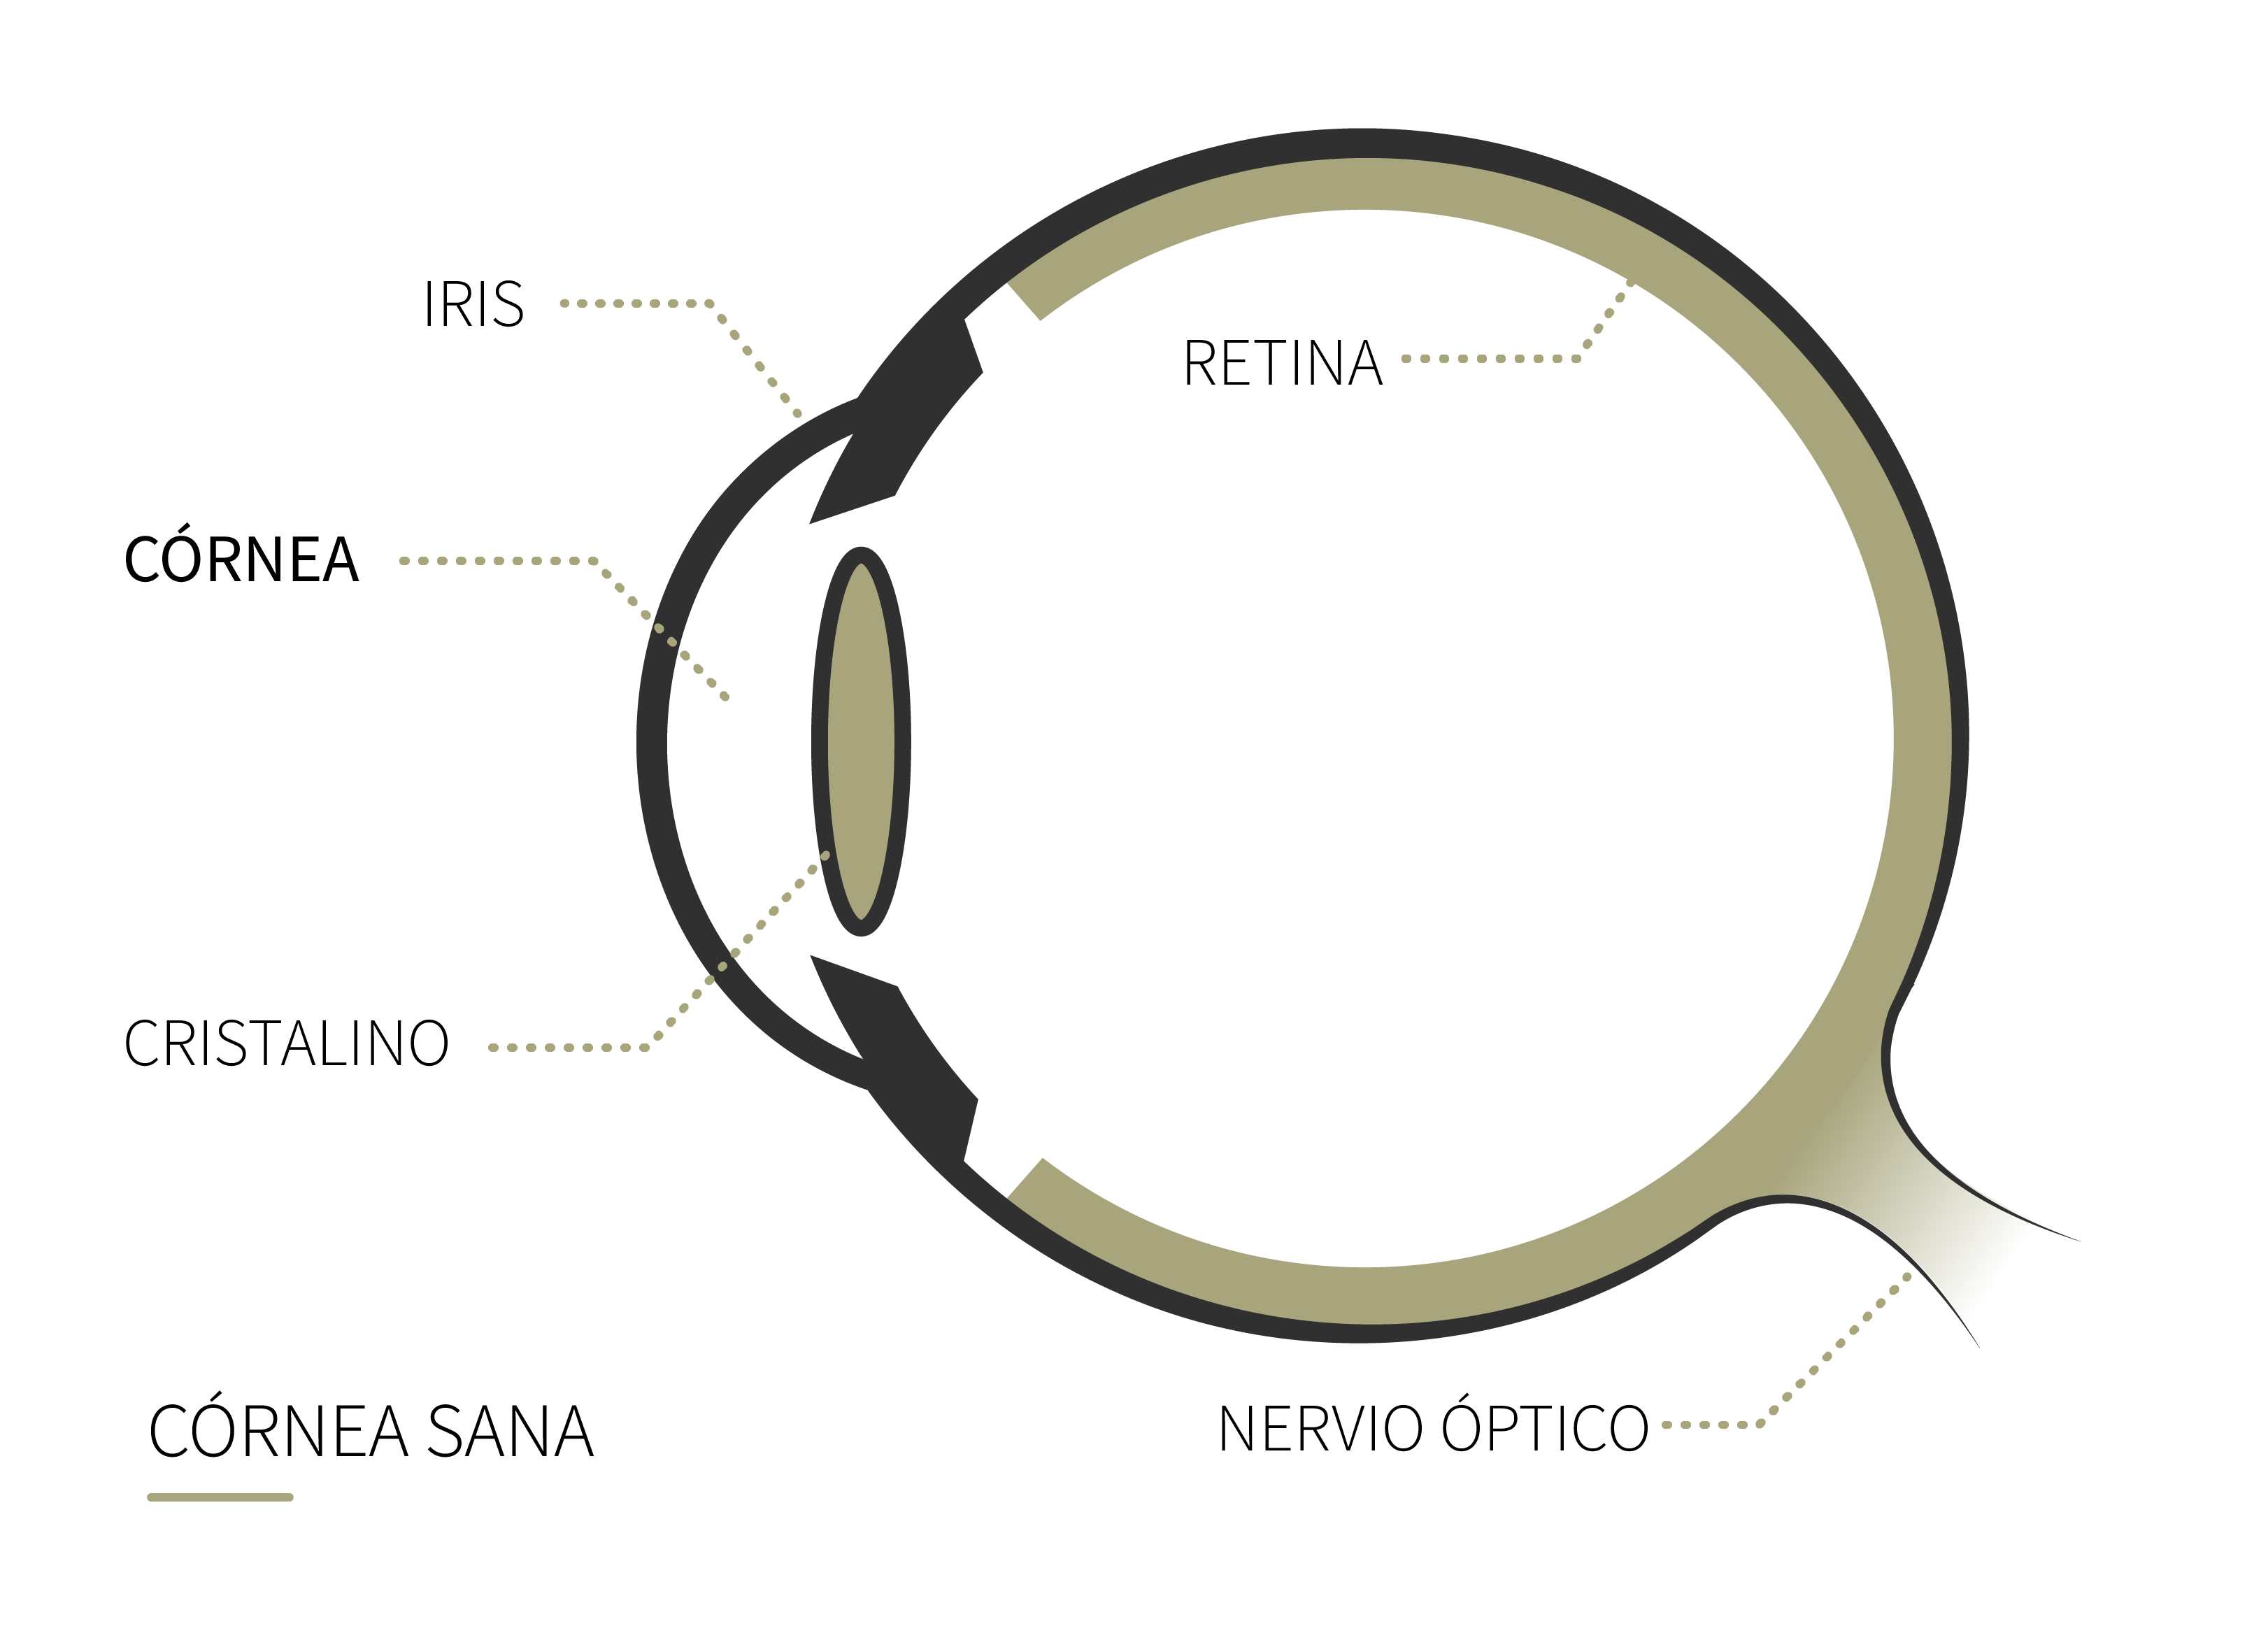
\includegraphics[width=\textwidth]{img/queratocono_deformacion_a.png}
                \caption{Córnea sana}
                \label{fig:cornea_a}
            \end{subfigure}
            \hspace{-1 cm}
            \begin{subfigure}[b]{0.45\textwidth} \centering
                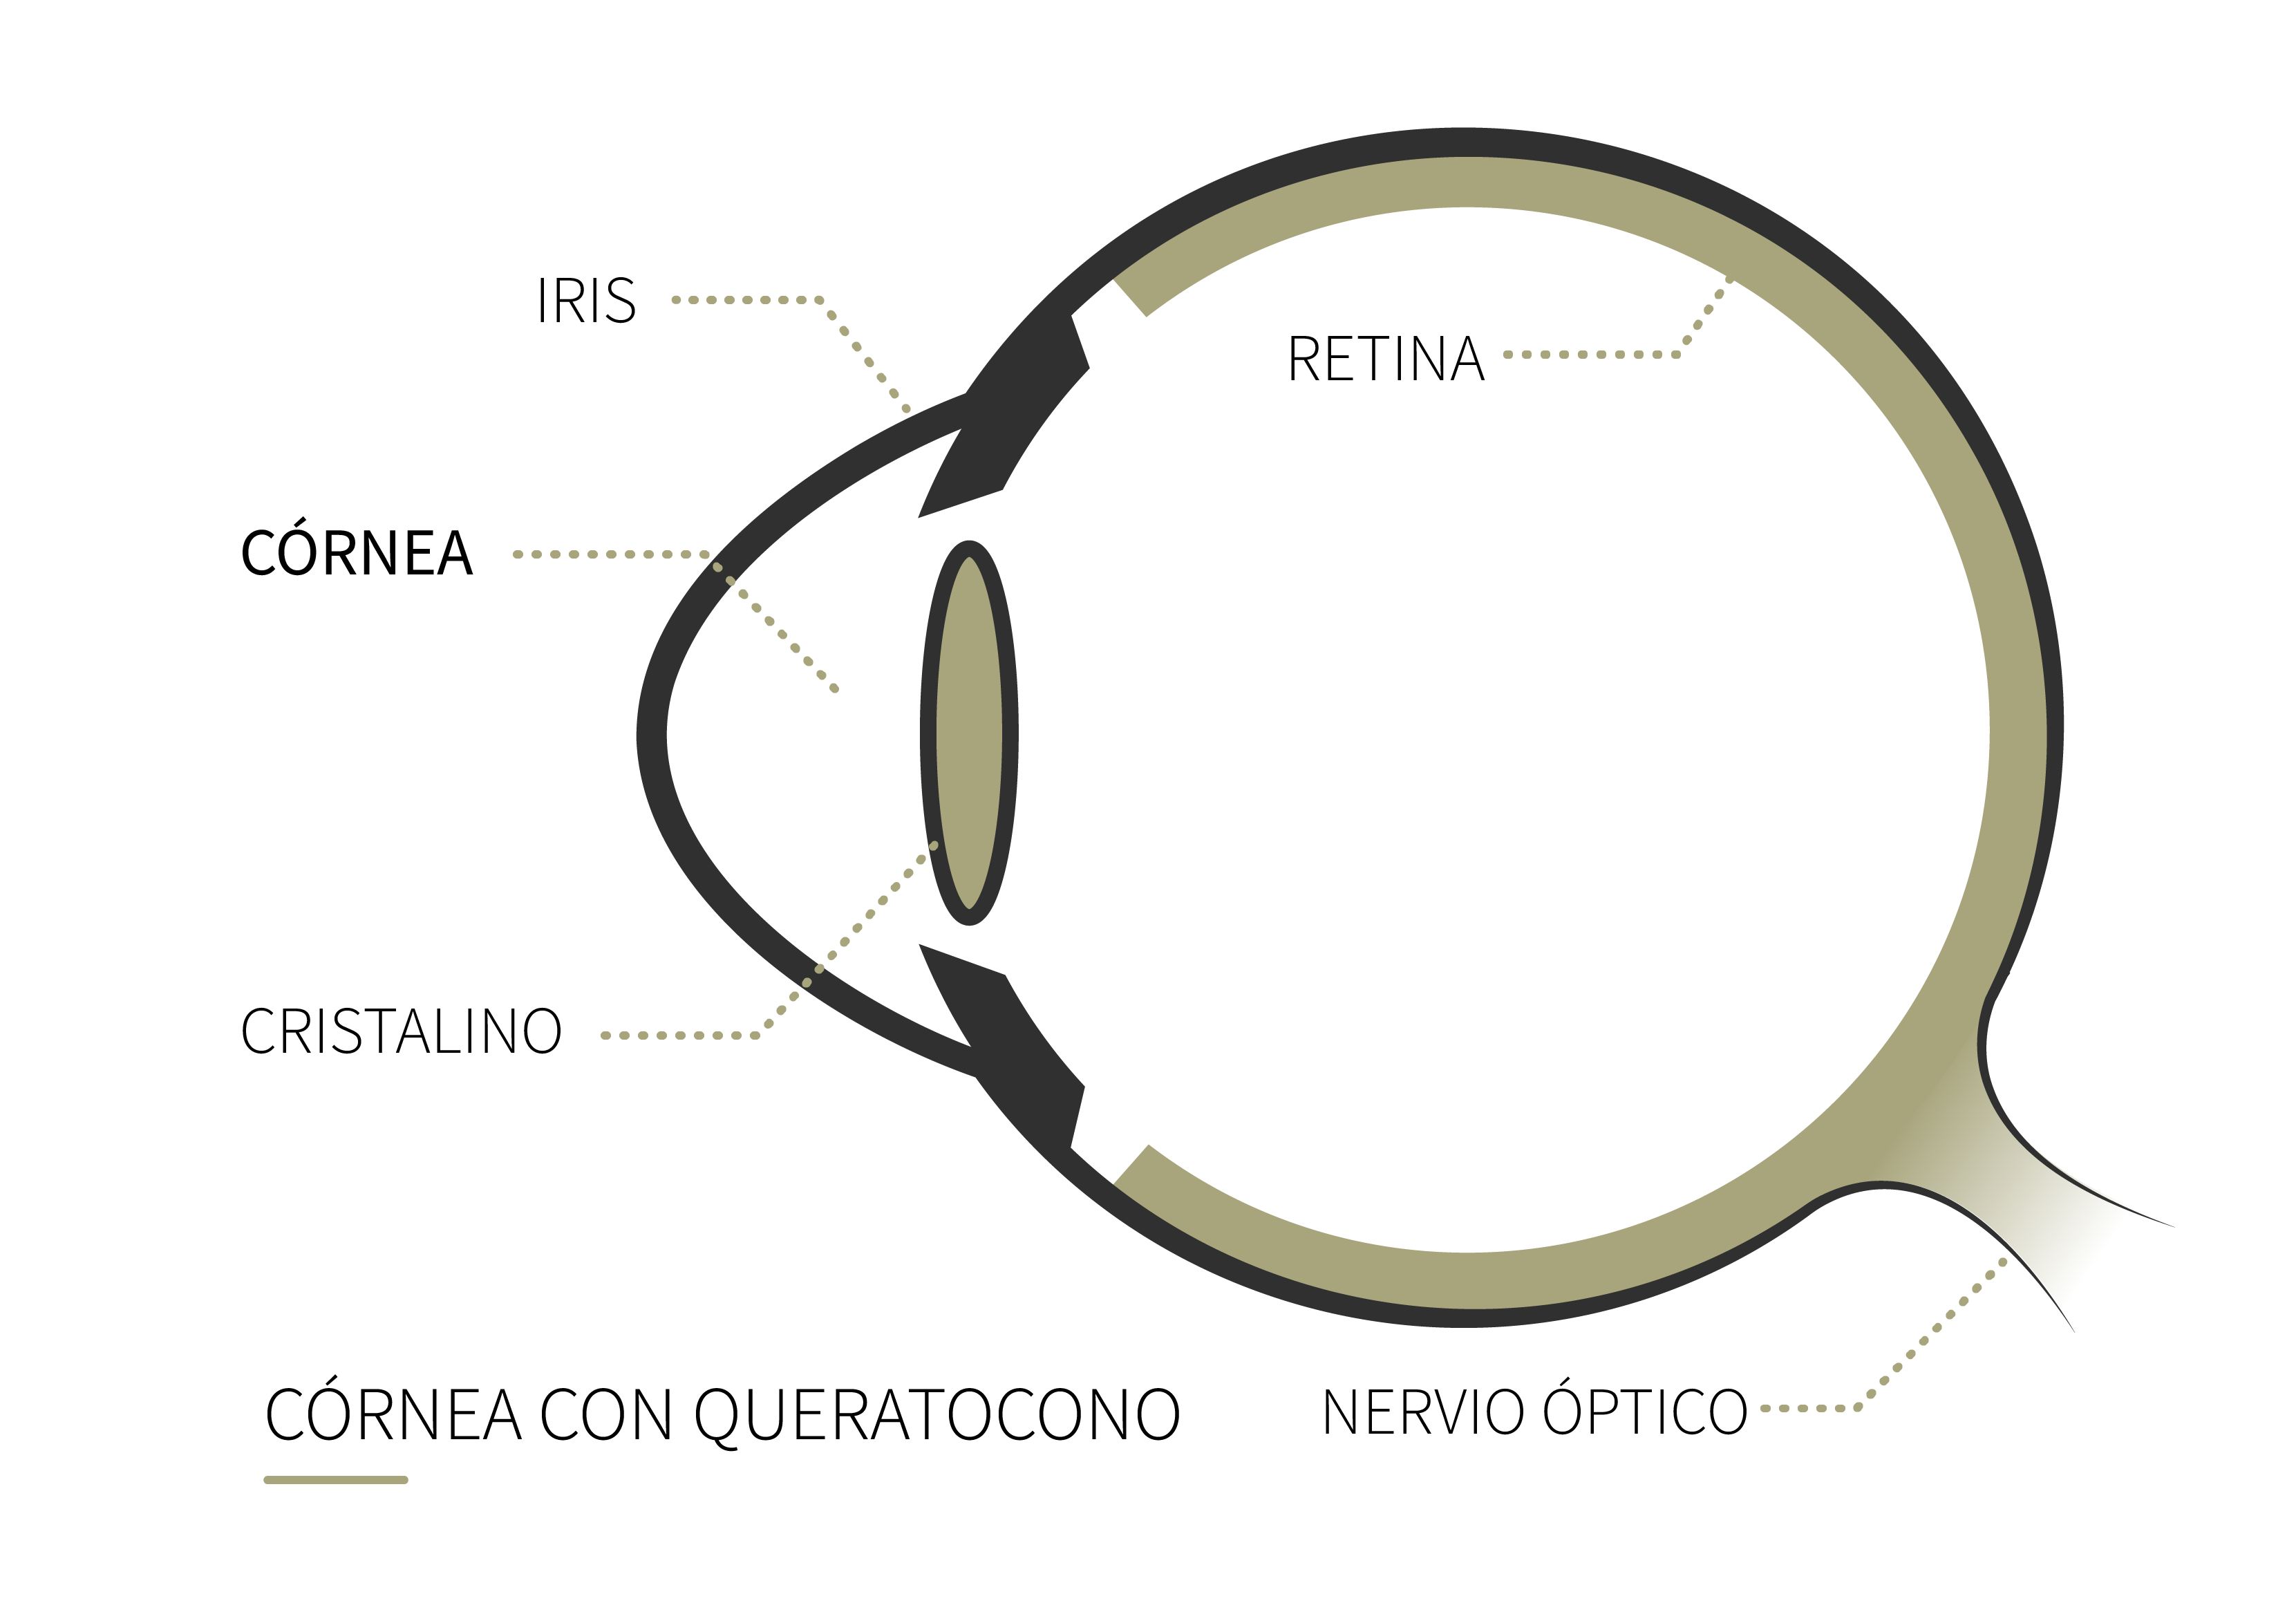
\includegraphics[width=\textwidth]{img/queratocono_deformacion_b.png}
                \caption{Córnea con queratocono}
                \label{fig:cornea_b}
            \end{subfigure}
            \caption{Comparación anatómica entre córnea sana y córnea con queratocono.}
            \label{fig:comparacion_corneas}
        \end{figure}

        La enfermedad se conoce desde hace más de dos siglos. Su primera descripción se atribuye a Burchard Mauchart en 1748, que la llamó \textit{staphyloma diaphanum}. En 1854, John Nottingham hizo la primera descripción detallada y la diferenció de otras enfermedades de la córnea~\cite{historia_kc}.

        La enfermedad tiene un inicio típico en la segunda década de la vida y puede progresar hasta la tercera o cuarta década, momento en el que generalmente se estabiliza~\cite{kcn_edad}.

        El diagnóstico se basa en la evaluación de múltiples parámetros corneales obtenidos mediante tomógrafos de Scheimpflug (como el Pentacam), topógrafos de Placido (como el Sirius) o sistemas de barrido por hendidura (como el Orbscan, con el que se obtuvieron los datos utilizados en este trabajo). Entre los parámetros clínicos más relevantes se encuentran la curvatura queratométrica (Km), el espesor corneal mínimo (paquimetría), el ``\textit{Differential Surface Elevation}'' (DSE) y los índices del sistema ABCD de Belin, que permite una estratificación de riesgo basada en la elevación anterior, la elevación posterior y el espesor corneal~\cite{kcn_parametros}.

    \phantomsection
    \subsection{Inteligencia Artificial en medicina: estado del arte}

        La aplicación de la Inteligencia Artificial en el ámbito médico ha experimentado un crecimiento exponencial en la última década, impulsada por la disponibilidad de grandes volúmenes de datos clínicos y el avance en técnicas de aprendizaje automático. En particular, los sistemas de soporte a la decisión clínica basados en IA han demostrado capacidad para asistir a los profesionales de salud en la interpretación de imágenes médicas, la estratificación de riesgo y la planificación de tratamientos~\cite{medicina_ia}. Estos sistemas no reemplazan al médico, sino que complementan su labor proporcionando un análisis objetivo y reproducible que puede ser verificado y validado por el especialista antes de tomar una decisión clínica.

        En el campo de la oftalmología, se han desarrollado múltiples modelos de IA para la detección de patologías oculares como la retinopatía diabética, el glaucoma y, más recientemente, el queratocono, como el modelo de Shafi Balal y KeratoDetect~\cite{shafi_balal,kerato_detect}. Sin embargo, la mayoría de estas soluciones se encuentran en fase de investigación y no han sido implementadas en sistemas operacionales reales, menos aún en contextos regionales como el de Misiones, donde la accesibilidad a equipos de diagnóstico de alta gama es limitada y la demanda de herramientas asistidas por tecnología es creciente.

    \phantomsection
    \subsection{Redes neuronales convolucionales para procesamiento de imágenes}

        Las redes neuronales convolucionales (CNN) representan la arquitectura de referencia para el procesamiento de imágenes. Su capacidad para extraer automáticamente características espaciales jerárquicas, desde bordes y texturas simples hasta patrones complejos, las convierte en herramientas idóneas para el análisis de mapas topográficos corneales.
        
        Estas redes utilizan capas de convolución que aplican filtros aprendidos a la imagen de entrada, seguidas de capas de agrupamiento (\textit{pooling}) que reducen la dimensionalidad preservando las características más relevantes. La profundidad de la red permite capturar niveles crecientes de abstracción, desde detalles de bajo nivel hasta estructuras de alto nivel, que podrían usarse para correlacionar patologías específicas.

        Entre las arquitecturas más utilizadas se encuentran \textit{EfficientNet-B7}, que ofrece un equilibrio óptimo entre precisión y eficiencia computacional mediante el escalado compuesto de profundidad, resolución y ancho de banda, siendo particularmente adecuado para imágenes médicas donde se requiere alta resolución para capturar detalles sutiles. \textit{ResNet}, por su parte, utiliza conexiones residuales que permiten entrenar redes muy profundas sin el problema de la degradación, facilitando la extracción de características de alta complejidad en imágenes de topografía corneal. 
        
        Por otro lado, los ViT constituyen una alternativa basada en mecanismos de atención que captura relaciones globales en la imagen, potencialmente útil para analizar la topografía corneal como un todo integrado. Para incorporar exportaciones de equipos de diferentes fabricantes, pueden emplearse algoritmos de visión artificial como \textit{YOLOv8} para la segmentación y recorte automático de las regiones de interés, llevándolas a una escala común antes de la entrada al modelo predictivo. En el prototipo esta etapa no resulta necesaria, ya que CornOrb provee los mapas ya recortados y estandarizados.

    \phantomsection
    \subsection{Aprendizaje profundo multimodal}

        El enfoque multimodal combina diferentes tipos de datos de entrada para mejorar la precisión diagnóstica. En el contexto del queratocono, esto implica integrar los mapas corneales, como los de elevación anterior y posterior, curvatura y paquimetría, con datos clínicos estructurados del paciente, como la edad, el astigmatismo, la curvatura máxima y el espesor corneal. En el caso de este trabajo, las fuentes son los cuatro mapas que provee el equipo Orbscan y las variables clínicas que los acompañan en el conjunto de datos utilizado.

        La combinación de estas fuentes de información permite al modelo capturar patrones que serían imperceptibles al analizar cada modalidad por separado. Por ejemplo, un mapa de elevación posterior puede mostrar una protrusión subclínica que, combinada con un espesor corneal reducido en una zona específica, fortalece la predicción de queratocono en etapas tempranas donde ninguno de los dos indicadores por sí solo resultaría concluyente.

        Una revisión sistemática sobre la combinación de imágenes médicas con datos de la historia clínica distingue tres estrategias de fusión, según el momento en que se unen ambas fuentes~\cite{huang_fusion}. En la fusión temprana, los datos se combinan antes de ingresar al modelo; en la fusión tardía, cada modalidad se analiza con un modelo independiente y solo se combinan sus predicciones finales; y en la fusión conjunta, una red convolucional extrae características de la imagen que se unen con las variables clínicas dentro de la misma red, de modo que ambas partes aprenden en simultáneo. Esta última es la estrategia adoptada en este trabajo: una rama convolucional procesa los mapas corneales, una rama de capas densas procesa los datos clínicos y una capa de fusión integra ambas representaciones antes de la clasificación final. Así, cada rama aprende las características más relevantes de su tipo de dato, mientras que la capa de fusión captura las interacciones entre ambos.

    \phantomsection
    \subsection{Modelos fundacionales y multimodales en oftalmología}

        Los modelos fundacionales son modelos de IA entrenados sobre volúmenes muy grandes y diversos de datos, en general sin etiquetas, mediante aprendizaje autosupervisado, es decir, aprendiendo a partir de la propia estructura de los datos. Una vez entrenados, pueden adaptarse a muchas tareas distintas con una cantidad reducida de datos etiquetados. En medicina, se plantea que estos modelos lleguen a interpretar de forma flexible distintas combinaciones de modalidades, como imágenes, historias clínicas, resultados de laboratorio o texto médico, dando lugar a una IA médica de propósito general~\cite{moor_gmai}.

        La oftalmología es una de las especialidades donde esta línea avanzó con mayor rapidez. RETFound, descrito en la sección Antecedentes, fue el primer modelo fundacional del área y trabaja exclusivamente con imágenes de retina~\cite{retfound}. Posteriormente, VisionFM extendió este enfoque a múltiples modalidades: fue preentrenado con 3,4 millones de imágenes de más de 500.000 personas, abarcando ocho tipos de estudios oftalmológicos (entre ellos retinografía, tomografía de coherencia óptica, lámpara de hendidura y ecografía), y alcanzó, en su validación interna, un área bajo la curva ROC promedio de 0,950 en el diagnóstico de ocho categorías de enfermedades oculares~\cite{visionfm}. Esta métrica mide la capacidad del modelo para distinguir casos sanos de casos enfermos, siendo 1 el valor ideal.

        Sin embargo, una revisión sistemática reciente de diez modelos fundacionales en oftalmología indica que ocho de ellos se centran en enfermedades de la retina, mientras que las aplicaciones al segmento anterior del ojo se limitan a tumores de la superficie ocular~\cite{jin_fm_oftalmologia}. La misma revisión señala como barreras para su adopción clínica la falta de interpretabilidad, la elevada demanda de cómputo, la integración con los sistemas clínicos existentes y la necesidad de validación por parte de los especialistas.

        Estos antecedentes son relevantes para el presente trabajo por dos motivos. En primer lugar, confirman el valor de combinar múltiples fuentes de información y de reutilizar conocimiento previamente aprendido, principios que el prototipo puede aplicar a menor escala: la rama convolucional puede partir de una red preentrenada (aprendizaje por transferencia) y se combina con los datos clínicos del paciente. En segundo lugar, muestran que los mapas de topografía corneal, centrales para el diagnóstico del queratocono, aún no forman parte de los modelos fundacionales disponibles. Por ello, y dado el volumen de datos y de cómputo que requieren, su desarrollo o adaptación para el queratocono se plantea como una línea de trabajo futuro (ver sección Alcance y limitaciones).

    \phantomsection
    \subsection{Explicabilidad de la Inteligencia Artificial (XAI)}

        La explicabilidad de la IA (XAI) es un componente crítico en sistemas de soporte a la decisión clínica, ya que permite al profesional médico comprender y verificar el razonamiento detrás de la predicción del algoritmo. Sin explicabilidad, los sistemas de IA se convierten en ``cajas negras'' que generan desconfianza en el usuario y dificultan su adopción, especialmente en un ámbito donde las decisiones tienen impacto directo en la salud. La explicabilidad no solo mejora la confianza, sino que también permite detectar posibles sesgos algorítmicos, ya que el profesional puede identificar si el modelo está enfocando su atención en regiones clínicamente relevantes o en partes de la imagen que no guardan relación con la patología.

        La técnica más utilizada en el ámbito de la visión artificial médica es Grad-CAM (\textit{Gradient-weighted Class Activation Mapping}), que genera mapas de calor que resaltan las regiones de la imagen que más influyeron en la decisión del modelo. En el contexto del queratocono, estos mapas permiten al oftalmólogo visualizar qué zonas corneales específicas activaron la predicción del algoritmo, proporcionando evidencia visual que fundamenta la decisión y facilita la validación por parte del especialista. La integración de XAI en el sistema propuesto no solo es una necesidad regulatoria, sino que constituye un diferencial técnico que posiciona al producto como una herramienta transparente y confiable para el uso clínico diario.

    \phantomsection
    \subsection{\textit{Software} como producto médico y marco regulatorio}

        El \textit{software} de soporte a la decisión clínica se enmarca conceptualmente como un SaMD, definido por la organización internacional de normalización (ISO) como \textit{software} destinado a ser utilizado con fines médicos sin formar parte de un \textit{hardware} médico. 
        
        En Argentina, la regulación de los SaMD está a cargo de la ANMAT, que establece las disposiciones N.º 2318/2002 y N.º 9688/2019~\cite{dispo_2318,dispo_9688} para la clasificación y registro de productos médicos. Según el nivel de riesgo asociado a la función que cumple el software, se clasifica en Clase I (bajo riesgo), Clase II (riesgo medio) o Clase III (alto riesgo).

        Para el proyecto propuesto, el registro como producto Clase II implica la necesidad de demostrar la seguridad y eficacia del sistema mediante validación clínica, así como el cumplimiento de la normativa de protección de datos personales (Ley N.º 25.326 (2000)~\cite{ley_25326}) para garantizar la anonimización de las muestras y el consentimiento informado de los pacientes. El cumplimiento normativo no es simplemente un requisito administrativo, sino que forma parte integral del diseño del sistema, ya que desde las etapas iniciales de desarrollo se deben implementar mecanismos de seguridad, trazabilidad y auditoría que permitan demostrar ante el organismo regulador que el producto cumple con los estándares de calidad y seguridad requeridos para su uso en el ámbito clínico.

    \phantomsection
    \subsection{Sistema ABCD de Belin para estratificación de riesgo}

        El sistema ABCD de Belin es un método de clasificación del queratocono que evalúa la córnea en cuatro dimensiones: A (elevación anterior), B (elevación posterior), C (curvatura corneal) y D (espesor corneal o paquimetría). Cada parámetro se puntúa en una escala que permite una estratificación objetiva de la severidad de la enfermedad y su riesgo de progresión. Este sistema supera las limitaciones del análisis convencional de mapas topográficos, que depende exclusivamente de la interpretación visual del especialista, ya que integra múltiples parámetros objetivos en una evaluación unificada, lo que facilita la comparabilidad de los resultados con estudios publicados y la aceptación del sistema por parte de la comunidad oftalmológica. Al basar la estratificación en un sistema validado y ampliamente reconocido, el proyecto se posiciona como una herramienta complementaria al flujo de trabajo clínico existente y no como un reemplazo del criterio médico especializado.

        Predecir los valores del sistema ABCD a partir de los mapas corneales permitiría que el sistema propuesto entregue, además de la detección, una clasificación de la severidad alineada con los estándares internacionales de diagnóstico. Sin embargo, entrenar un modelo con ese fin requiere estudios etiquetados con dichos índices, con los que no cuenta el conjunto de datos utilizado. Por este motivo, la estratificación basada en el sistema ABCD se plantea como una línea de trabajo futuro (ver sección Alcance y limitaciones).

\phantomsection
\section{Propuesta metodológica}

    La propuesta se adapta a la metodología CRISP-DM combinada con un desarrollo incremental, dado que el proyecto avanza mediante ciclos iterativos de entendimiento y preparación de datos, modelado, evaluación y despliegue, en lugar de seguir un esquema secuencial clásico tipo cascada.

    La planificación distingue dos horizontes. El primero corresponde al PFI y abarca las dos primeras fases, que culminan en el prototipo descrito en la sección Alcance y limitaciones. El segundo corresponde a la proyección del producto: las fases tres y cuatro, necesarias para llevar el prototipo al uso clínico y comercial, y que quedan fuera del alcance del PFI.

    Para el PFI se establece una línea base de cuatro meses, de octubre de 2026 a enero de 2027, en concordancia con la duración de un cuatrimestre. A esta línea base se suma una reserva de contingencia de hasta dos meses (febrero y marzo de 2027), destinada a absorber los retrasos que puedan surgir por la naturaleza iterativa del modelado o por la materialización de los riesgos identificados en la sección Gestión de riesgos.

    \subsection*{Primera fase: datos y modelo}

        La primera fase abarca los meses uno a tres (octubre a diciembre de 2026) y se centra en la preparación de los datos y el desarrollo del modelo. Desde su inicio se definen los requisitos regulatorios, legales y de calidad, estableciendo las políticas de documentación y trazabilidad que exigirá la futura inscripción del sistema como producto médico, de modo que el registro de cada decisión se lleve en paralelo al desarrollo y no deba reconstruirse al final.

        Se parte del análisis exploratorio del \textit{dataset} CornOrb~\cite{zenodo}, cuyos resultados se presentan en el capítulo Desarrollo, y se preparan los datos para el entrenamiento. Luego se experimenta con arquitecturas multimodales que combinan una rama convolucional para los mapas corneales con una rama para las variables clínicas. El modelo seleccionado se entrena y se evalúa con la partición de entrenamiento y prueba que provee el propio \textit{dataset}, priorizando la reducción de los falsos negativos, y se le integra la técnica Grad-CAM para generar la explicación visual de cada predicción.

        En paralelo, se avanza con las solicitudes de muestras locales anonimizadas a centros oftalmológicos de la región. Si se obtienen durante esta fase, se utilizan para una primera evaluación del modelo sobre datos regionales; el lote completo se destina a la validación clínica prevista en la tercera fase.

    \subsection*{Segunda fase: aplicación web}

        La segunda fase abarca los meses tres y cuatro (diciembre de 2026 y enero de 2027), solapándose con el cierre de la primera. En ella el modelo se encapsula en una aplicación web: se desarrolla el \textit{backend}, encargado de la lógica del servidor y de exponer el modelo mediante una API construida con el \textit{framework} FastAPI, y el \textit{frontend}, la interfaz con la que interactúa el oftalmólogo, desarrollada con React.

        La aplicación permite cargar los estudios de un paciente, ejecutar el modelo y consultar un informe con el resultado, el nivel de confianza y el mapa de calor que lo justifica. Además, incorpora la gestión de usuarios necesaria para el modelo de suscripción y se despliega en un servidor VPS para su prueba.

    \subsection*{Proyección del producto}

        Una vez finalizado el PFI, la llegada del sistema al uso clínico y comercial requiere dos fases adicionales, cada una con una duración estimada de dos meses.

        La tercera fase corresponde a la validación clínica y las pruebas de usuario. Se verifica el desempeño del modelo con un conjunto de alrededor de 150 estudios locales no utilizados durante el entrenamiento, calculando un intervalo de confianza del 90\,\% sobre las métricas de sensibilidad y especificidad, y se realizan ajustes de la interfaz a partir de pruebas de usabilidad con personal médico.

        La cuarta fase corresponde a la certificación regulatoria y el lanzamiento. Se cierra el informe técnico elaborado a lo largo de todo el desarrollo y, con el acompañamiento de un abogado consultor, se gestiona la inscripción del sistema como producto médico Clase II ante la ANMAT. Asimismo, se aprueban los contratos de confidencialidad, los términos de uso con limitación de responsabilidad clínica y los consentimientos informados, en cumplimiento de la Ley N.º 25.326 (2000) de Protección de los Datos Personales. Por último, se ejecuta la campaña de comunicación del producto y se elabora la documentación técnica y el manual de usuario.

        Sumando el PFI (incluida su reserva de contingencia) y estas dos fases, el desarrollo completo del producto se extiende por diez meses, con el lanzamiento comercial a partir del mes once. Este horizonte es el que se toma como base para el análisis económico del capítulo Análisis de Producto de Mercado.

    \vspace{0.25 cm}
    \subsection{Cronograma de actividades}

        La Tabla~\ref{tabla:cronograma} resume la distribución temporal de las fases, y el detalle de las actividades se presenta en el Diagrama de Gantt de la Figura~\ref{fig:anexo_gantt}, por mes. En azul, las actividades del PFI (de octubre de 2026 a enero de 2027); en gris, la reserva de contingencia (febrero y marzo de 2027); y en naranja, las fases de la proyección del producto.

        \begingroup \setstretch{1.1}
        \begin{longtblr}[
            caption = Distribución temporal de las fases del proyecto,
            label = tabla:cronograma
            ]{
                colspec = {X[l,m] Q[c,m,1.6cm] Q[c,m,5.4cm] Q[c,m,2.2cm]},
                cells = {font=\small},
                row{1} = {bg=gray!15, font=\small\bfseries, halign=c},
                hlines, vlines,
                rowsep = 3pt, colsep = 5pt
            }

            Fase & Meses & Período & Horizonte \\

            Primera fase: datos y modelo & 1 a 3 & octubre a diciembre de 2026 & PFI \\

            Segunda fase: aplicación web & 3 y 4 & diciembre de 2026 y enero de 2027 & PFI \\

            Reserva de contingencia & 5 y 6 & febrero y marzo de 2027 & PFI \\

            Tercera fase: validación clínica & 7 y 8 & --- & Producto \\

            Cuarta fase: certificación y lanzamiento & 9 y 10 & --- & Producto \\

        \end{longtblr}
        \endgroup


    % Desarrollo
    % \newpage
\phantomsection
\chapter{Desarrollo}

\phantomsection
\section{Relevamiento clínico y análisis exploratorio de datos (EDA)}

    Tal como se planteó en la primera fase de la propuesta metodológica, se estableció contacto con diferentes centros de salud y profesionales del área de oftalmología, con el fin de reunir muestras locales anonimizadas que permitan evaluar el modelo con datos de la región. Las solicitudes se encuentran en curso y, hasta que se concreten, el trabajo continúa sobre los datos públicos del \textit{dataset} CornOrb, disponible en Zenodo~\cite{zenodo}.

    \phantomsection
    \subsection{Centros de salud y profesionales contactados}

        Los centros de salud y profesionales contactados hasta la fecha se detallan en la Tabla~\ref{tabla:centros_contactados}. Además de centros de Misiones, se incluyeron instituciones de otras provincias y del exterior, con el objetivo de ampliar las posibilidades de obtener muestras.

        \begingroup \setstretch{1.1}
        \begin{longtblr}[
            caption = Centros de salud y profesionales de oftalmología contactados,
            label = tabla:centros_contactados
            ]{
                colspec = {X[l,m] Q[l,m,4cm]},
                cells = {font=\small},
                row{1} = {bg=gray!15, font=\small\bfseries, halign=c},
                hlines, vlines,
                rowsep = 3pt, colsep = 5pt
            }

            Centro de salud o profesional & Ubicación \\

            Centro de Ojos Misiones Alta Complejidad & Posadas \\

            Clínica de Ojos Cáceres Zorrilla & Posadas \\

            Clínica de Ojos Maldonado Bas & Córdoba \\

            Universidad Hospital Italiano & Buenos Aires \\

            Dr. Óscar Mallo & Buenos Aires \\

            Clínica de Ojos Córdoba & Córdoba \\

            Clínica de Ojos Dr. Nano & Buenos Aires \\

            Clínica Vidavas & Perú \\

            Clínica de Ojos Dr. Santiago Barreyro & Posadas \\

        \end{longtblr}
        \endgroup

        Estos contactos constituyen el punto de partida para conformar el lote de muestras locales anonimizadas previsto en la propuesta metodológica. Si las muestras se obtienen durante el PFI, se utilizarán para una primera evaluación del modelo con datos de la región; su uso para una validación clínica formal corresponde a la proyección del producto (ver sección Alcance y limitaciones).

    \phantomsection
    \subsection{Conjunto de datos de trabajo}

        Mientras se concretan las solicitudes de muestras locales, el análisis se realiza sobre el \textit{dataset} CornOrb~\cite{zenodo}. Este recurso reúne 1.454 registros correspondientes a ojos de 744 pacientes, estudiados con un equipo Orbscan~3 en centros de oftalmología de Argelia. Para cada ojo se proporcionan cuatro mapas corneales (axial, anterior, posterior y paquimetría) en formato de imagen, junto con un archivo de datos clínicos que incluye la etiqueta diagnóstica: normal o queratocono. Según la documentación del \textit{dataset}, las etiquetas fueron asignadas por oftalmólogos, y los datos se encuentran anonimizados.

        El \textit{dataset} incluye además una partición predefinida de los registros: el 80\,\% se destina al entrenamiento del modelo y el 20\,\% restante se reserva para su evaluación final. A su vez, la porción de entrenamiento está dividida en cinco subconjuntos (\textit{folds}) para realizar validación cruzada, es decir, entrenar y evaluar el modelo cinco veces rotando la porción que se deja afuera, de modo de obtener una estimación más estable de su desempeño.

        La Tabla~\ref{tabla:variables_cornorb} describe las variables clínicas que acompañan a cada registro.

        \begingroup \setstretch{1.1}
        \begin{longtblr}[
            caption = Variables clínicas del \textit{dataset} CornOrb,
            label = tabla:variables_cornorb
            ]{
                colspec = {Q[l,m,4.7cm] X[l,m] Q[c,m,2cm]},
                cells = {font=\small},
                row{1} = {bg=gray!15, font=\small\bfseries, halign=c},
                hlines, vlines,
                rowsep = 3pt, colsep = 5pt
            }

            Variable & Descripción & Unidad \\

            \texttt{age\_years} & Edad del paciente & años \\

            \texttt{gender} & Sexo del paciente (femenino o masculino) & --- \\

            \texttt{eye} & Ojo estudiado (derecho u izquierdo) & --- \\

            \texttt{astig\_value\_D} & Astigmatismo corneal & dioptrías \\

            \texttt{kmax\_value\_D} & Curvatura máxima de la córnea (K max), indicador clásico de queratocono & dioptrías \\

            \texttt{pachy\_central\_um} & Espesor de la córnea en su centro (paquimetría central) & µm \\

            \texttt{pachy\_thinnest\_um} & Espesor de la córnea en su punto más delgado & µm \\

            \texttt{pachy\_thinnest\_x}, \texttt{\_y} & Ubicación del punto más delgado & mm \\

            \texttt{asphericity\_anterior}, \texttt{\_posterior} & Asfericidad de las superficies anterior y posterior: cuánto se aparta la forma de la córnea de una esfera & --- \\

            \texttt{astig\_axis\_deg}, \texttt{kmax\_axis\_deg} & Orientación del astigmatismo y de la curvatura máxima & grados \\

            \texttt{label} & Etiqueta diagnóstica: 0 = normal, 1 = queratocono & --- \\

        \end{longtblr}
        \endgroup

    \phantomsection
    \subsection{Análisis exploratorio de datos}

        El análisis exploratorio de datos (EDA) tiene como objetivo conocer la composición y la calidad del conjunto de datos antes de entrenar el modelo, para detectar problemas que puedan sesgar los resultados y orientar las decisiones de preprocesamiento. Se realizó en Python con las bibliotecas \textit{pandas}, \textit{matplotlib}, \textit{seaborn} y \textit{scipy}.

        \subsubsection*{Calidad de los datos}

            El archivo de datos clínicos no presenta valores faltantes ni filas duplicadas. Para cada uno de los ojos se encontraron los cuatro mapas corneales, con un total de 5.628 imágenes. Sin embargo, se identificaron los siguientes aspectos a depurar antes del entrenamiento:

            \begin{itemize}[leftmargin=*]
                \item \textbf{Mediciones repetidas:} 46 ojos cuentan con más de una medición, lo que representa 47 registros adicionales. No son copias exactas, sino estudios distintos del mismo ojo, por lo que debe decidirse si se conservan como muestras independientes o se agrupan.

                \item \textbf{Inconsistencia de nombres:} el código de un paciente figura como \texttt{3E+132} en el archivo de datos y como \texttt{3E132} en la carpeta de imágenes, probablemente porque una planilla de cálculo lo interpretó como un número en notación científica. Hasta corregirlo, los dos ojos de ese paciente no pueden vincularse con sus imágenes.

                \item \textbf{Valores atípicos:} se registran valores de K max de 4,0 y 4,9 dioptrías, que no son posibles en una córnea real (los valores normales rondan las 44 dioptrías) y probablemente correspondan a errores de carga. También se observa al menos un registro con un espesor mínimo mayor al espesor central (615~µm frente a 524~µm), lo que es contradictorio por definición.
            \end{itemize}

        \subsubsection*{Composición del conjunto de datos}

            El 61,14\,\% de los registros corresponde a ojos normales y el 38,86\,\% a ojos con queratocono (Figura~\ref{fig:eda_clases}). Existe, por lo tanto, un desbalance moderado de aproximadamente 1,57 ojos normales por cada ojo con queratocono. Este desbalance no es extremo, pero obliga a evaluar el modelo con métricas que reflejen su desempeño sobre la clase minoritaria, como la sensibilidad, y no solo con el porcentaje global de aciertos.

            \begin{figure}[H]
                \centering
                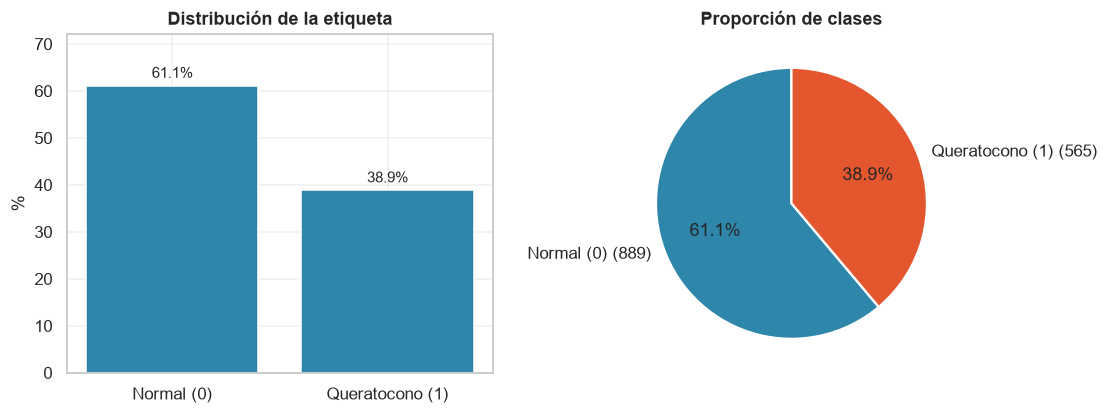
\includegraphics[width=0.85\linewidth]{img/eda/eda_clases.png}
                \caption{Distribución de los registros según la etiqueta diagnóstica.}
                \label{fig:eda_clases}
            \end{figure}

            La partición predefinida conserva esta proporción tanto en el conjunto de entrenamiento (61,13\,\% y 38,87\,\%) como en el de evaluación (61,17\,\% y 38,83\,\%), y los cinco \textit{folds} tienen un tamaño similar, de entre 230 y 236 registros cada uno.

            Dado que un mismo paciente puede aportar ambos ojos, se verificó que ningún paciente aparezca a la vez en el conjunto de entrenamiento y en el de evaluación. Esta condición se cumple, lo que evita una fuga de información, si los dos ojos de un paciente quedaran repartidos entre ambos conjuntos, el modelo sería evaluado sobre un paciente que ya ``conoció'' durante el entrenamiento, y su desempeño resultaría artificialmente alto. Además, la etiqueta es la misma para todos los registros de un paciente.

        \subsubsection*{Variables demográficas}

            El 65,13\,\% de los registros corresponde a mujeres y el 34,87\,\% a hombres, mientras que los ojos derecho e izquierdo están prácticamente balanceados (50,21\,\% y 49,79\,\%).

            La edad media es de 33,5 años en el grupo normal y de 27,9 años en el grupo con queratocono, cuyo registro más joven tiene 13 años (Figura~\ref{fig:eda_edad}). Este resultado es coherente con lo planteado en el Marco teórico respecto de la aparición temprana de la enfermedad~\cite{kcn_edad}, aunque describe a la muestra del \textit{dataset} y no a la población general.

            \begin{figure}[H]
                \centering
                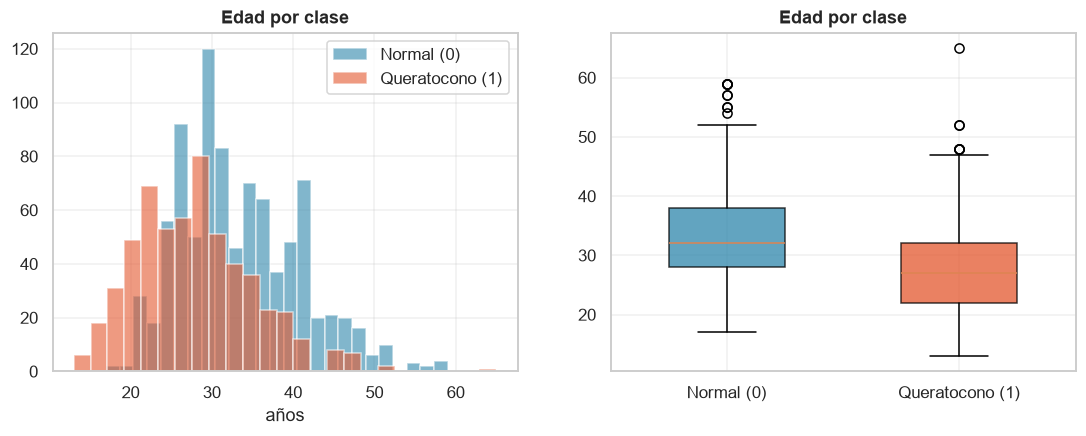
\includegraphics[width=0.85\linewidth]{img/eda/eda_edad.png}
                \caption{Distribución de la edad de los pacientes según la etiqueta diagnóstica.}
                \label{fig:eda_edad}
            \end{figure}

            En cuanto al sexo, al contar ojos, la proporción de queratocono resulta mayor en mujeres (40,76\,\%) que en hombres (35,31\,\%), con una diferencia estadísticamente significativa (prueba de chi-cuadrado, p\,=\,0,048). Sin embargo, al repetir el análisis contando pacientes, la diferencia se reduce (40,76\,\% frente a 38,81\,\%) y deja de ser relevante (p\,=\,0,658). El resultado inicial era, en parte, un efecto de contar los dos ojos de un mismo paciente como casos independientes. Se concluye que no hay evidencia de que un sexo tenga mayor probabilidad de queratocono en este \textit{dataset}. Aun así, como la muestra tiene mayoría de mujeres, conviene informar el desempeño del modelo por separado para cada sexo, para verificar que no favorezca a ninguno.

        \subsubsection*{Variables clínicas}

            La Figura~\ref{fig:eda_variables_clinicas} compara la distribución de cada variable clínica entre ambos grupos. En cada gráfico, la caja abarca la mitad central de los valores y la línea interior marca la mediana. Los ojos con queratocono presentan una curvatura máxima mayor (K max medio de 53,1 frente a 43,7 dioptrías), una córnea más delgada (espesor mínimo medio de 427,5 frente a 520,7~µm), mayor astigmatismo y una asfericidad más negativa, es decir, una córnea que se aparta más de la forma esférica. Estas diferencias coinciden con la descripción clínica de la enfermedad presentada en el Marco teórico.

            \begin{figure}[H]
                \centering
                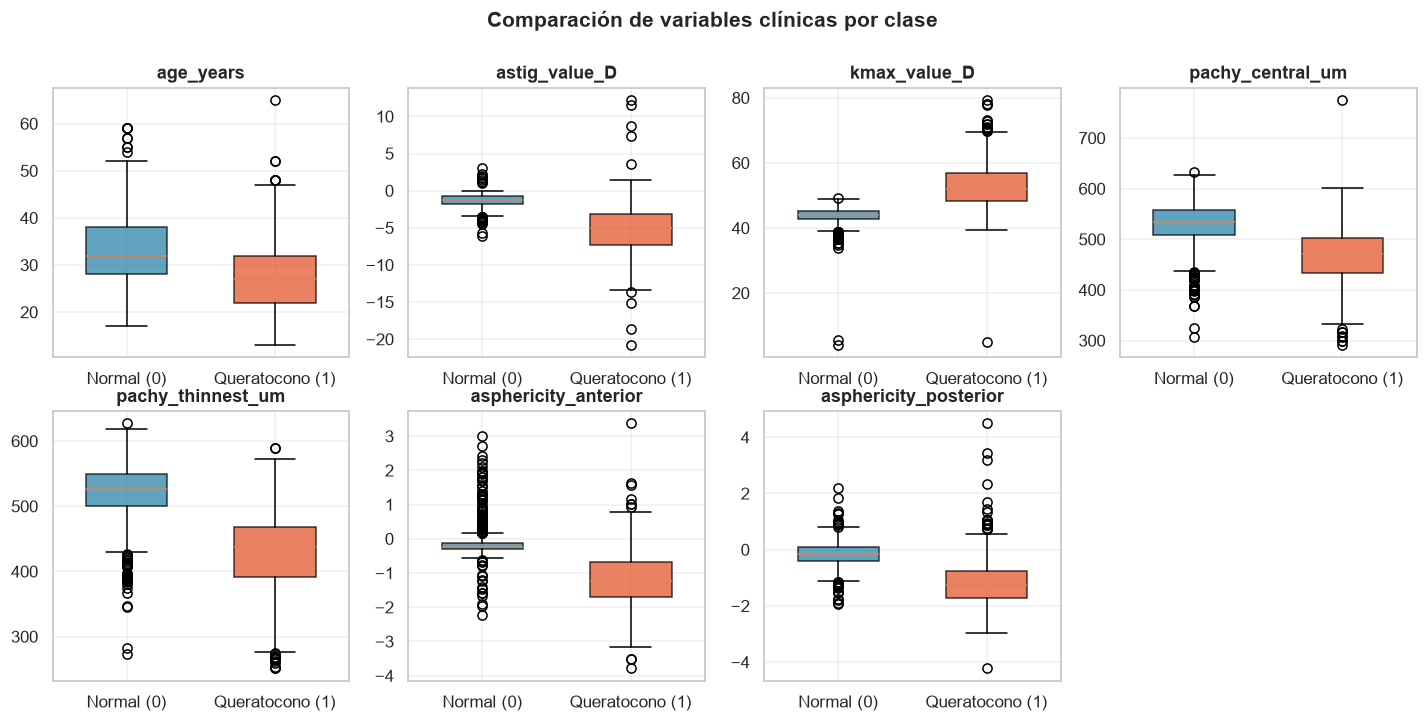
\includegraphics[width=\linewidth]{img/eda/eda_variables_clinicas.png}
                \caption{Comparación de las variables clínicas entre ojos normales y ojos con queratocono.}
                \label{fig:eda_variables_clinicas}
            \end{figure}

            Para cuantificar qué tanto se relaciona cada variable con el diagnóstico, se calculó su correlación con la etiqueta (Figura~\ref{fig:eda_correlacion}). La correlación toma valores entre \textminus{}1 y 1: cuanto más se aleja de cero, más se diferencia esa variable entre ojos normales y ojos con queratocono, y su signo indica si el valor aumenta o disminuye con la enfermedad. Las variables más relacionadas son el K max (0,69), el espesor mínimo (\textminus{}0,67), el astigmatismo (\textminus{}0,66) y la asfericidad anterior (\textminus{}0,64) y posterior (\textminus{}0,62), mientras que la ubicación del punto más delgado aporta poca información.

            \begin{figure}[H]
                \centering
                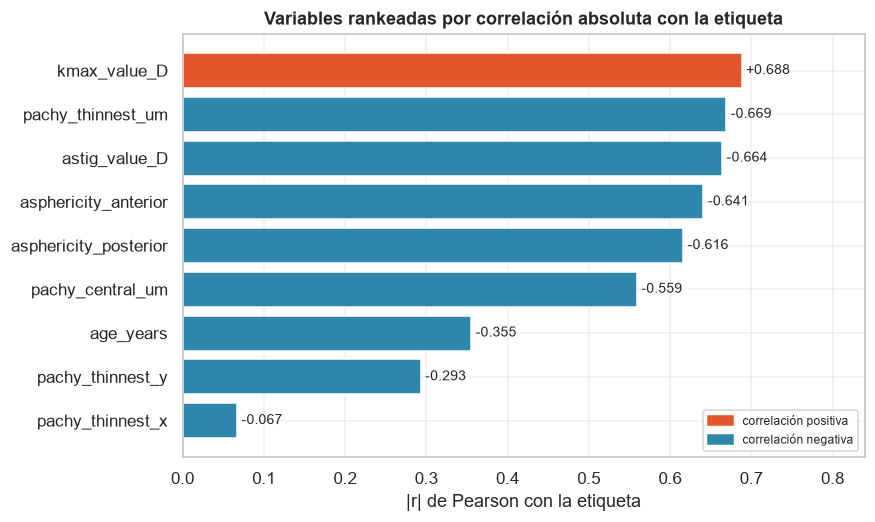
\includegraphics[width=0.68\linewidth]{img/eda/eda_correlacion.png}
                \caption{Variables clínicas ordenadas según su correlación con la etiqueta diagnóstica.}
                \label{fig:eda_correlacion}
            \end{figure}

            Muchas de estas variables también están relacionadas entre sí, ya que describen distintos aspectos de una misma deformación de la córnea. Esto debe tenerse en cuenta en el modelado para evitar que el modelo dependa de información redundante.

        \subsubsection*{Conclusiones del análisis}

            El análisis confirma que el \textit{dataset} es adecuado como punto de partida para el prototipo: tiene una partición bien construida, sin fugas de información entre pacientes, y sus variables clínicas muestran diferencias claras entre ojos normales y ojos con queratocono. Esto respalda la decisión de construir un modelo multimodal, en el que una rama analice estas variables junto a la rama que procesa los mapas corneales. Del análisis se desprenden las siguientes decisiones para la etapa de modelado:

            \begin{itemize}[leftmargin=*]
                \item Corregir el código de paciente \texttt{3E+132} y depurar los valores atípicos identificados antes del entrenamiento.

                \item Definir el tratamiento de las mediciones repetidas de un mismo ojo.

                \item Respetar la partición y los \textit{folds} predefinidos, de modo que los ojos de un mismo paciente queden siempre en el mismo conjunto.

                \item Evaluar el modelo priorizando la sensibilidad, en línea con el objetivo de reducir los falsos negativos, e informar su desempeño por separado para cada sexo.

                \item Transformar las variables de orientación (ejes en grados) antes de utilizarlas, ya que, por ejemplo, 1° y 179° representan orientaciones casi idénticas pese a la diferencia numérica.
            \end{itemize}
    

    % Estudio financiero
    \newpage
\phantomsection
\chapter{Estudio financiero}

    Este capítulo determina la viabilidad económica y financiera de KERALYTIX. Las primeras secciones resumen el estudio de mercado, la factibilidad, el presupuesto y la gestión de riesgos, que sirven de contexto. La sección Viabilidad económica y financiera define luego cómo se financia el proyecto y calcula el precio final, la TREMA, el VAN y la TIR, siguiendo los criterios de la Guía de costos y evaluación de factibilidad del proyecto~\cite{guia_costos}.

\section{Estudio de mercado}

    \phantomsection
    \subsection{Usuarios y usos}

        Sus usuarios de KERALYTIX son los oftalmólogos generales, los especialistas en córnea y los técnicos de centros de optometría de alta complejidad de Misiones que cuentan con equipos de topografía o tomografía corneal.

        \begin{figure}[H]
            \centering
            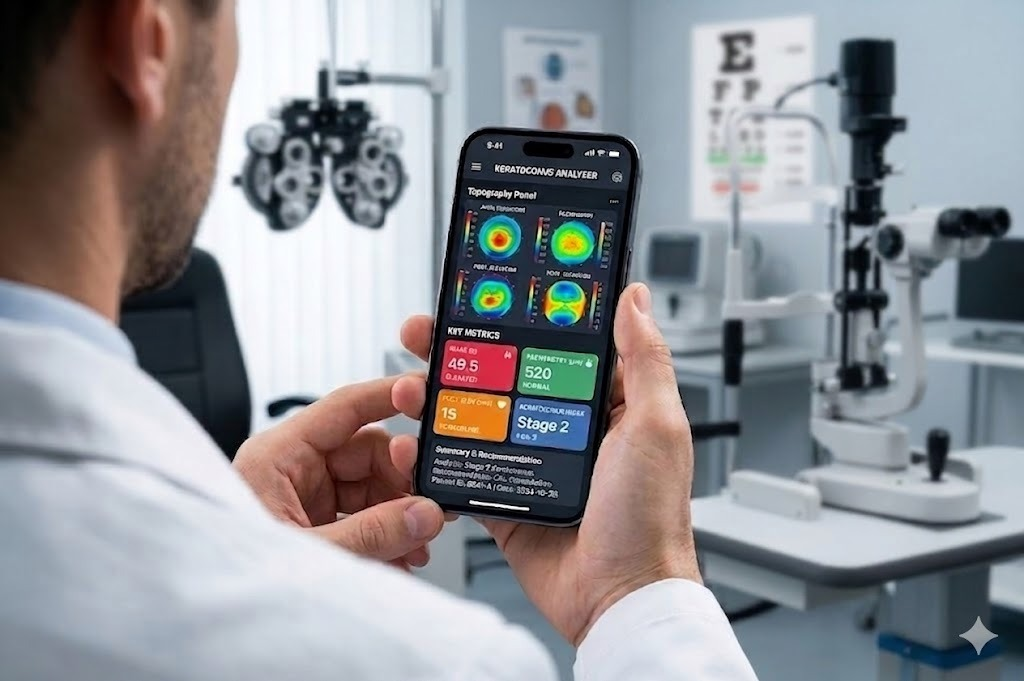
\includegraphics[width=0.5\linewidth]{img/humo.jpeg}
            \caption{Representación visual de la aplicación.}
        \end{figure}

    \phantomsection
    \subsection{Análisis de demanda}

        Existe una necesidad creciente de una herramienta de este tipo derivada de la naturaleza subjetiva del análisis de los estudios. La Tabla~\ref{tabla:demanda} resume los factores que la sustentan.

        \begingroup \setstretch{1.1}
        \vspace{0.3cm}\noindent\begin{talltblr}[
            caption = Factores que sustentan la demanda de KERALYTIX,
            label = tabla:demanda
            ]{
                colspec = {Q[l,m,3.4cm] X[l,m] Q[c,m,2.4cm]},
                cells = {font=\small},
                row{1} = {bg=gray!15, font=\small\bfseries, halign=c},
                hlines, vlines,
                rowsep = 3pt, colsep = 5pt
            }

            Factor & Sustento & Fuente \\

            Subjetividad diagnóstica & La interpretación depende de la experiencia del oftalmólogo, lo que aumenta los errores en etapas subclínicas, que se confunden con enfermedades más comunes. & \cite{deteccion_temprana} \\

            Volumen local de casos & Aumento reportado de casos de queratocono en Oberá, que requieren un diagnóstico preciso. & \cite{misiones} \\

            Descentralización de la atención & Una primera evaluación asistida permite derivar a los centros de alta complejidad solo los casos que lo requieren. & Análisis del problema \\

            Marco normativo & Disposiciones de la ANMAT que encuadran el \textit{software} como producto médico y respaldan la modernización tecnológica en salud. & \cite{dispo_2318,dispo_9688} \\

        \end{talltblr}\par\vspace{0.3cm}
        \endgroup

    \phantomsection
    \subsection{Análisis de la oferta}

        El mercado está dominado por un grupo reducido de fabricantes que venden sistemas cerrados, cuyo \textit{software} de análisis solo funciona con sus propios equipos y no emite una predicción diagnóstica. En el país no existen competidores directos con un \textit{software} como producto médico específico para queratocono. Los aportes y las limitaciones de cada alternativa se resumen en la Tabla~\ref{tabla_antecedentes_comparativa} del capítulo Contextualización.

    \phantomsection
    \subsection{Análisis de precios}

        La Tabla~\ref{tabla:precios_competencia} compara la forma de cobro de la competencia con la de KERALYTIX, y la Tabla~\ref{tabla:estructura_costos} resume la estructura de costos sobre la que se define el precio final (ver sección Viabilidad económica y financiera).

        \begingroup \setstretch{1.1}
        \vspace{0.3cm}\noindent\begin{talltblr}[
            caption = Comparativa de precios de la oferta competitiva,
            label = tabla:precios_competencia
            ]{
                colspec = {Q[l,m,3.8cm] X[l,m] X[l,m]},
                cells = {font=\small},
                row{1} = {bg=gray!15, font=\small\bfseries, halign=c},
                hlines, vlines,
                rowsep = 3pt, colsep = 5pt
            }

            Competidor & Inversión inicial & Modelo de facturación \\

            Sistemas tradicionales (OCULUS / Ziemer) & USD 20.000 a USD 40.000 por equipo, con el \textit{software} incluido & Licencia cerrada, ligada al equipo \\

            Referente local de IA (Entelai) & No requiere \textit{hardware} propio & Pago por informe: $\approx$\,\$\,3.790 + IVA~\cite{entelai} \\

            \textbf{KERALYTIX} & No requiere \textit{hardware} nuevo: procesa los mapas que exportan los equipos existentes & Suscripción mensual de \$\,180.000 por centro \\

        \end{talltblr}\par\vspace{0.3cm}
        \endgroup

        \vspace{-0.5 cm}
        \begingroup \setstretch{1.1}
        \vspace{0.3cm}\noindent\begin{talltblr}[
            caption = Estructura de costos de KERALYTIX,
            label = tabla:estructura_costos
            ]{
                colspec = {X[l,m] Q[c,m,3.2cm] Q[r,m,3.4cm]},
                cells = {font=\small},
                row{1} = {bg=gray!15, font=\small\bfseries, halign=c},
                hlines, vlines,
                rowsep = 3pt, colsep = 5pt
            }

            Concepto & Tipo de costo & Monto \\

            Servidor VPS (desde el mes 7) & Fijo mensual & \$\,41.600 \\

            Herramientas de desarrollo: Claude Code y Google Colab Pro (años 2 a 6) & Fijo mensual & \$\,49.300 \\

            Monotributo categoría A de los dos integrantes~\cite{monotributo_2026} & Fijo mensual & \$\,99.054 \\

            Cuotas de los dos créditos del Fondo de Crédito Misiones (meses 4 a 60) & Fijo mensual & \$\,295.617 \\

            Inversión pre-operativa del primer año (desarrollo, validación y habilitación ante la ANMAT) & Única & \$\,13.872.740 \\

            Atención de un suscriptor adicional & Variable & $\approx$\,\$\,0 \\

        \end{talltblr}\par\vspace{0.3cm}
        \endgroup

        El costo variable por suscriptor es prácticamente nulo, porque un mismo servidor atiende a varios centros. Por eso, una vez cubiertos los costos fijos, cada suscripción adicional se transforma casi por completo en ganancia.

    \phantomsection
    \subsection{Análisis de la comercialización}

        La estrategia de comercialización se basa en un servicio digital escalable, que se integra al flujo de trabajo actual del oftalmólogo como complemento de su equipamiento. La Tabla~\ref{tabla:comercializacion} resume sus componentes.

        \begingroup \setstretch{1.1}
        \begin{longtblr}[
            caption = Estrategia de comercialización de KERALYTIX,
            label = tabla:comercializacion
            ]{
                colspec = {Q[l,m,3.4cm] X[l,m]},
                cells = {font=\small},
                row{1} = {bg=gray!15, font=\small\bfseries, halign=c},
                hlines, vlines,
                rowsep = 3pt, colsep = 5pt
            }

            Aspecto & Estrategia \\

            Producto requerido & Interoperable, capaz de recibir imágenes de distintos equipos; intuitivo, con una interfaz que no requiera conocimientos de IA; y fiable, con evidencia visual (XAI) que sustente la decisión clínica. \\

            Mensaje central & Una ``segunda opinión'' que estandariza el diagnóstico, reduce la subjetividad y previene errores en etapas subclínicas. \\

            Difusión científica & Publicación de los resultados de la validación con datos locales en congresos de oftalmología o informática. \\

            Marketing directo & Presentaciones institucionales en clínicas privadas de Misiones, el Ministerio de Salud Pública y otros interesados. \\

            Presencia digital & Difusión en redes profesionales (LinkedIn), \textit{newsletters} del sector salud y \textit{webinars} técnicos. \\

            Distribución y acceso & Aplicación web desplegada en un servidor VPS, con acceso por suscripción desde el navegador de cualquier dispositivo. \\

            Canales de venta & Venta directa a instituciones de salud, alianzas con distribuidores de equipamiento oftalmológico (como complemento de sus equipos) y asistencia técnica remota. \\

        \end{longtblr}
        \endgroup

    \phantomsection
    \subsection{Estudio de factibilidad y viabilidad del proyecto}

        La factibilidad se evaluó con cuatro criterios ponderados: técnico (40\,\%), jurídico (25\,\%), operativo (20\,\%) y económico (15\,\%). Los aspectos que considera cada criterio se detallan en la Tabla~\ref{tabla:anexo_criterios} y el análisis de cada uno en la Tabla~\ref{tabla:anexo_analisis_criterios}, ambas en el Anexo. La Tabla~\ref{tabla:viabilidad} resume el resultado.

        \begingroup \setstretch{1.1}
        \vspace{0.3cm}\noindent\begin{talltblr}[
            caption = Resumen de la evaluación de viabilidad del proyecto,
            label = tabla:viabilidad
            ]{
                colspec = {Q[l,m,2.6cm] Q[c,m,1.6cm] Q[c,m,2.2cm] X[l,m]},
                cells = {font=\small},
                row{1} = {bg=gray!15, font=\small\bfseries, halign=c},
                hlines, vlines,
                rowsep = 3pt, colsep = 5pt
            }

            Criterio & Peso & Evaluación & Principal condicionante \\

            Técnica & 40\,\% & Alta & Compatibilidad limitada a equipos Orbscan en el prototipo \\

            Jurídica & 25\,\% & Media & La inscripción ante la ANMAT requiere validación clínica \\

            Operativa & 20\,\% & Favorable & Aceptación a confirmar en pruebas con usuarios \\

            Económica & 15\,\% & Media & Depende del aporte propio y de la aprobación de dos créditos del Fondo de Crédito Misiones \\

        \end{talltblr}\par\vspace{0.3cm}
        \endgroup

        En síntesis, el criterio de mayor peso, la viabilidad técnica, es también el más favorable, lo que respalda la factibilidad del prototipo planteado para el PFI. Los condicionantes jurídicos y económicos recaen principalmente sobre la proyección del producto: los primeros se abordan en la planificación y en la gestión de riesgos, y los segundos se analizan en la sección Viabilidad económica y financiera.

\vspace{-0.5 cm}
\phantomsection
\section{Presupuesto}

    El presupuesto del primer año de KERALYTIX asciende a \$\,15.774.992 y se resume por rubro en la Tabla~\ref{tabla:presupuesto_resumen}. El desarrollo se realiza en el ámbito de la Facultad de Ingeniería de Oberá (UNaM), que cubre el espacio de trabajo y los servicios básicos, por lo que no se presupuestan alquileres. Los recursos humanos propios reciben una retribución simbólica basada en el Salario Mínimo, Vital y Móvil~\cite{cita:SMVM}, y de las 40 horas de consultoría oftalmológica previstas, la mitad se cubre mediante un convenio académico que ofrece coautoría en las publicaciones científicas. El congreso nacional de oftalmología se traslada al segundo año, cuando el proyecto ya registra ingresos.

    \begingroup \setstretch{1.1}
    \vspace{0.3cm}\noindent\begin{talltblr}[
        caption = Resumen del presupuesto del primer año por rubro,
        label = tabla:presupuesto_resumen
        ]{
            colspec = {Q[l,m,3.6cm] X[l,m] Q[r,m,2.6cm] Q[c,m,1.3cm] Q[c,m,1.6cm]},
            cells = {font=\small},
            row{1} = {bg=gray!15, font=\small\bfseries, halign=c},
            row{8} = {bg=gray!15, font=\small\bfseries},
            hlines, vlines,
            rowsep = 3pt, colsep = 5pt
        }

        Rubro & Detalle & Monto & \% & Detalle en \\

        Recursos materiales & Dos computadoras portátiles & \$\,4.200.000 & 26,6 & Tabla~\ref{tabla:anexo_recursos_materiales} \\

        Recursos humanos propios & Pasantes desarrolladores de IA y web & \$\,3.876.400 & 24,6 & Tabla~\ref{tabla:rrhh_propios} \\

        Recursos humanos adicionales & Diseño UX/UI y marketing digital & \$\,642.000 & 4,1 & Tabla~\ref{tabla:rrhh_adicionales} \\

        Consultoría y servicios & Oftalmólogo (horas pagas), abogado, Google Colab y Claude Code & \$\,3.559.240 & 22,6 & Tabla~\ref{tabla:consultoria_servicios} \\

        Movilidad, logística y matriculación & Traslados, aranceles de la ANMAT y congreso (año 2) & \$\,2.059.100 & 13,0 & Tabla~\ref{tabla:otros_costos} \\

        Costos operativos del primer año & Servidor VPS (6 meses) y monotributo de los integrantes (12 meses) & \$\,1.438.252 & 9,1 & Tabla~\ref{tabla:estructura_costos} \\

        \SetCell[c=2]{r} TOTAL & & \$\,15.774.992 & 100 & \\

    \end{talltblr}\par\vspace{0.3cm}
    \endgroup

    De este total, \$\,13.872.740 corresponden a la inversión pre-operativa del primer año, \$\,464.000 al congreso del segundo año y el resto a los costos operativos. Las tablas detalladas de cada rubro se presentan en el Anexo.

\phantomsection
\section{Gestión de riesgos}

    Cada riesgo se evalúa según su probabilidad de ocurrencia y su gravedad, en escalas de 1 a 5 (Tablas~\ref{riesgos_prob} y~\ref{riesgos_grav} del Anexo). El producto de ambas da el impacto (Tabla~\ref{riesgos_imp}), que se clasifica como bajo (0 a 7), medio (8 a 13) o alto (14 a 25). A los ocho riesgos identificados en la planificación se suman tres asociados al esquema de financiamiento (R9 a R11). La Tabla~\ref{riesgos} resume la clasificación, y la descripción y los planes de acción de cada riesgo se presentan en la Tabla~\ref{tabla:anexo_planes_riesgos} del Anexo.

    \begingroup \setstretch{1.1}
    \vspace{0.3cm}\noindent\begin{talltblr}[
        caption = Riesgos y clasificación de los mismos,
        label = riesgos
        ]{
            colspec = {Q[c,m,1cm] X[l,m] Q[c,m,2cm] Q[c,m,2cm] Q[c,m,2cm] Q[c,m,2cm]},
            cells = {font=\small},
            row{1} = {bg=gray!15, font=\small\bfseries, halign=c},
            hlines, vlines,
            rowsep = 3pt, colsep = 5pt
        }

        ID & Riesgo identificado & Ocurrencia & Gravedad & Impacto & Riesgo \\

        R1 & Sesgo y falta de generalización      & 3 & 5 & 15 & Alto  \\
        R2 & Incompatibilidad de formatos         & 4 & 4 & 16 & Alto  \\
        R3 & Dificultades con los datos locales   & 4 & 5 & 20 & Alto  \\
        R4 & Fallas en la integración             & 4 & 2 & 8  & Medio \\
        R5 & Subestimación de costos              & 4 & 3 & 12 & Medio \\
        R6 & Demora de la certificación           & 3 & 2 & 6  & Bajo  \\
        R7 & Resistencia de adopción              & 3 & 2 & 6  & Bajo  \\
        R8 & Diferencias entre los integrantes    & 2 & 1 & 2  & Bajo  \\
        R9 & Rechazo o reducción de uno de los créditos & 3 & 4 & 12 & Medio \\
        R10 & Cuotas sin ingresos suficientes     & 3 & 5 & 15 & Alto  \\
        R11 & Fondos no aplicables al destino previsto & 3 & 3 & 9 & Medio \\

    \end{talltblr}\par\vspace{0.3cm}
    \endgroup

    Los riesgos en la etapa comercia R10 es el más relevante, si el lanzamiento o la captación de suscriptores se demoran, las cuotas siguen venciendo y la deuda queda respaldada por los garantes. Por eso el aporte propio se dimensiona para cubrir el peor momento de caja con un margen (ver Flujo de caja con financiamiento).

    \phantomsection
    \subsection{Impacto temporal}

        La materialización de los riesgos afecta de forma distinta al cronograma (Tabla~\ref{tabla:impacto_temporal}). R1, R2 y R3 tienen una afectación directa: pueden obligar a volver a la etapa de desarrollo o bloquear el inicio de la validación clínica. R4, R5, R7 y R8 tienen una afectación acotada o indirecta, y R6 no compromete el desarrollo técnico, porque solo posterga el uso clínico formal.

        Los riesgos financieros afectan sobre todo al inicio y a la etapa comercial. R9 y R11 pueden demorar el desembolso y, con él, las compras del primer mes, mientras que R10 no modifica el cronograma técnico, pero compromete la caja de los años 2 y 3.

        \begingroup \setstretch{1.1}
        \vspace{0.3cm}\noindent\begin{talltblr}[
            caption = Impacto temporal de los riesgos identificados,
            label = tabla:impacto_temporal
            ]{
                colspec = {Q[c,m,1cm] Q[c,m,2.6cm] X[l,m]},
                cells = {font=\small},
                row{1} = {bg=gray!15, font=\small\bfseries, halign=c},
                hlines, vlines,
                rowsep = 3pt, colsep = 5pt
            }

            ID & Afectación & Etapa y efecto \\

            R1 & Directa & Validación clínica: el reentrenamiento focalizado implica volver a la etapa de desarrollo. \\
            R2 & Directa & Desarrollo, si obliga a rehacer el preprocesamiento, o validación, si un centro usa un formato no contemplado. \\
            R3 & Directa & Bloquea el inicio de la validación clínica local hasta resolverse. \\
            R4 & Acotada & Integración: el desarrollo modular y Docker permiten aislar los errores. \\
            R5 & Indirecta & Certificación y lanzamiento, si se activa la búsqueda de financiamiento externo. \\
            R6 & Nula sobre el desarrollo & Posterga solo el uso clínico formal y comercial. \\
            R7 & Acotada & Reduce los casos de la validación; demora solo si hay que sumar centros. \\
            R8 & Menor & Tareas puntuales del equipo, sin comprometer las etapas generales. \\
            R9 & Indirecta & Inicio del proyecto: demora el desembolso y las compras del mes 1. \\
            R10 & Nula sobre el desarrollo & Etapa comercial: compromete la caja de los años 2 y 3. \\
            R11 & Indirecta & Inicio del proyecto: obliga a reformular el destino de los fondos. \\

        \end{talltblr}\par\vspace{0.3cm}
        \endgroup

        Cabe destacar que la validación clínica con muestras locales forma parte de la proyección del producto, por lo que R1 y R3 no bloquean la entrega producto mínimo viable. Para los riesgos que sí pueden afectarlo, como R2, R4 y R8, el cronograma prevé la reserva de contingencia de hasta dos meses descrita en la propuesta metodológica.

\phantomsection
\section{Viabilidad económica y financiera}
\label{sec:viabilidad_economica}

    Según la Guía de costos~\cite{guia_costos}, un proyecto es viable cuando su Valor Actual Neto (VAN) es positivo y su Tasa Interna de Retorno (TIR) supera la Tasa de Rendimiento Mínima Aceptable (TREMA). Esta sección define primero cómo se financia KERALYTIX y luego calcula esos indicadores. Se toma un horizonte de seis años y los flujos se expresan a precios constantes de octubre de 2026.

    \phantomsection
    \subsection{Fuentes de financiamiento}

        Durante los primeros diez meses KERALYTIX no tiene un producto comercializable, por lo que no registra ingresos. El equipo cuenta con un capital inicial reducido, así que se relevaron las líneas vigentes del Fondo de Crédito Misiones (FCM)~\cite{fcm_faq,fcm_lineas}, resumidas en la Tabla~\ref{tabla:lineas_fcm}.

        \begingroup \setstretch{1.1}
        \vspace{0.3cm}\noindent\begin{talltblr}[
            caption = Líneas de crédito del Fondo de Crédito Misiones analizadas,
            label = tabla:lineas_fcm
            ]{
                colspec = {Q[l,m,2.4cm] X[l,m] Q[l,m,2.5cm] Q[l,m,2.6cm] Q[l,m,2.6cm]},
                cells = {font=\footnotesize},
                row{1} = {bg=gray!15, font=\footnotesize\bfseries, halign=c},
                row{2} = {bg=yellow!10},
                hlines, vlines,
                rowsep = 3pt, colsep = 4pt
            }

            Línea & Destinatarios & Monto & Tasa, plazo y gracia & ¿Aplica a KERALYTIX? \\

            Despegue Emprendedor~\cite{fcm_despegue} & Emprendimientos a iniciarse: no inscriptos, monotributistas, responsables inscriptos y personas jurídicas & Hasta \$\,6.000.000, hasta el 100\,\% del proyecto & 60\,\% de la TAMAR, fija (15\,\% en octubre de 2026); hasta 60 meses y 3 de gracia & Sí. No exige facturación previa \\

            Competitividad PyMEs~\cite{fcm_competitividad} & Pymes con al menos un año de trayectoria & De \$\,4.000.000 a \$\,200.000.000, hasta el 80\,\% del proyecto & 28\,\% fija el primer año, luego TAMAR + 2 puntos; hasta 48 meses y 6 de gracia de capital & No por ahora. Podría usarse desde el año 2 o 3 para crecer \\

            Línea de hasta \$\,20.000.000 con garantías reales (2025)~\cite{fcm_montos_2025} & Emprendimientos con hipoteca, prenda o aval bancario & Hasta \$\,20.000.000 & Sin datos publicados & No vigente: desde 2026 el monto no depende de la garantía \\

        \end{talltblr}\par\vspace{0.3cm}
        \endgroup

        \noindent\colorbox{yellow!10}{%
            \parbox{\dimexpr\linewidth-2\fboxsep}{%
                \par\noindent\colorbox{gray!15}{%
            \parbox{\dimexpr\linewidth-2\fboxsep}{%
                \setlength{\parindent}{1.5em}\indent
                El préstamo de \$\,20.000.000 al 28\,\% con seis meses de gracia que se había planteado inicialmente combinaba el monto de la línea de 2025 con las condiciones de Competitividad PyMEs, y no es accesible en el primer año. Según las preguntas frecuentes del FCM, el tipo de garantía ya no influye en el monto, los proyectos nuevos tienen un tope de \$\,6.000.000, y los montos mayores requieren al menos un año de trayectoria~\cite{fcm_faq}. Además, Competitividad PyMEs solo financia el 80\,\% del proyecto y, para garantías reales, pide la declaración jurada de IVA de los últimos doce meses~\cite{fcm_requisitos_cfi}.
            }%
        }
            }%
        }
        

        Por lo tanto, el esquema elegido combina \textbf{dos créditos Despegue Emprendedor}, uno por integrante (\$\,12.000.000 en total), con un \textbf{aporte propio de \$\,8.500.000} proveniente de ahorros de los integrantes y de aportes familiares. La Tabla~\ref{tabla:destino_fondos} detalla qué rubros puede cubrir el crédito según los destinos que admite el FCM, que no financia sueldos ni honorarios salvo los de investigación y desarrollo (I+D)~\cite{fcm_faq}.

        \begingroup \setstretch{1.1}
        \begin{longtblr}[
            caption = Destino de los fondos y fuente de financiamiento de cada rubro,
            label = tabla:destino_fondos
            ]{
                colspec = {X[l,m] Q[r,m,2.4cm] Q[l,m,4.2cm] Q[c,m,1.8cm]},
                cells = {font=\small},
                row{1} = {bg=gray!15, font=\small\bfseries, halign=c},
                row{7,15} = {bg=gray!15, font=\small\bfseries},
                hlines, vlines,
                rowsep = 3pt, colsep = 5pt
            }

            Rubro & Monto & Encuadre en el FCM & Fuente \\

            Computadoras portátiles & \$\,4.200.000 & Activo fijo, financiable & Crédito \\

            Consultoría oftalmológica (validación clínica) & \$\,2.580.000 & Honorarios de I+D, financiables a confirmar & Crédito \\

            Pasantes desarrolladores de IA y web & \$\,3.876.400 & Honorarios de I+D, financiables a confirmar & Crédito \\

            Diseño de interfaces UX/UI & \$\,480.000 & Honorarios de I+D, financiables a confirmar & Crédito \\

            Suscripciones de \textit{software} y servidor VPS & \$\,841.200 & Capital de trabajo, devolución en 12 meses & Crédito \\

            \SetCell[c=1]{r} Subtotal cubierto con los créditos & \$\,11.977.600 & & \\

            Habilitación y registro ante la ANMAT & \$\,1.575.100 & Arancel regulatorio, no previsto & Aporte \\

            Consultoría legal & \$\,387.640 & Honorarios, no financiables & Aporte \\

            Marketing digital & \$\,162.000 & Publicidad, no financiable & Aporte \\

            Traslados a la clínica colaboradora & \$\,20.000 & No financiable & Aporte \\

            Monotributo de los integrantes (año 1) & \$\,1.188.652 & No financiable & Aporte \\

            Cuotas de los créditos (año 1) & \$\,3.110.556 & No financiable & Aporte \\

            Reserva para los déficits de caja del año 2 & \$\,2.056.052 & No financiable & Aporte \\

            \SetCell[c=1]{r} Subtotal cubierto con el aporte propio & \$\,8.500.000 & & \\

        \end{longtblr}
        \endgroup

    \phantomsection
    \subsection{Condiciones del crédito y requisitos}

        La Tabla~\ref{tabla:condiciones_despegue} resume las condiciones de la línea Despegue Emprendedor vigentes en octubre de 2026 y los requisitos que deberá cumplir cada integrante.

        \begingroup \setstretch{1.1}
        \begin{longtblr}[
            caption = Condiciones y requisitos de la línea Despegue Emprendedor (octubre de 2026),
            label = tabla:condiciones_despegue
            ]{
                colspec = {Q[l,m,3.4cm] X[l,m]},
                cells = {font=\small},
                row{1} = {bg=gray!15, font=\small\bfseries, halign=c},
                hlines, vlines,
                rowsep = 3pt, colsep = 5pt
            }

            Aspecto & Condición \\

            Monto & Hasta \$\,6.000.000 por solicitante y hasta el 100\,\% del proyecto~\cite{fcm_despegue}. \\

            Tasa de interés & 60\,\% de la TAMAR, fija durante todo el crédito; 15\,\% anual en octubre de 2026. Se fija en el mes en que se firma el contrato~\cite{fracran_despegue}. \\

            Plazo y gracia & Hasta 60 meses, con hasta 3 meses de gracia. Se modelan 3 meses en los que solo se pagan intereses (\$\,75.000 por crédito) y 57 cuotas. \\

            Sistema de amortización & Francés, con cuotas mensuales que vencen el día 10. Cuota de \$\,147.809 por crédito (\$\,295.617 entre ambos). \\

            Garantías & A sola firma, fianza o seguro de caución~\cite{fcm_despegue}; las preguntas frecuentes del FCM admiten también prenda, hipoteca y avales de FOGAMI o de una SGR~\cite{fcm_faq}. \\

            Destinos financiables & Activo fijo (maquinaria, herramientas, mobiliario) y capital de trabajo; honorarios solo si corresponden a investigación y desarrollo. El capital de trabajo se devuelve en un máximo de 12 meses~\cite{fcm_faq}. \\

            Destinos excluidos & Sueldos, alquileres, publicidad (salvo construcción de marca), cancelación de deudas, celulares y rodados no utilitarios, entre otros~\cite{fcm_faq}. \\

            Requisitos del solicitante & Inscripción en ARCA (monotributo) y en Ingresos Brutos ante la ATM antes de firmar; situación crediticia normal en los últimos dos años; DNI y certificado de domicilio; formulario del proyecto, anexo fotográfico y presupuestos de los bienes; manifestación de bienes; CBU propio~\cite{fcm_requisitos}. \\

            Localización y habilitación & Acreditar el lugar del emprendimiento (alquiler, título o comodato) y presentar la habilitación municipal, definitiva o en trámite~\cite{fcm_requisitos}. \\

            Trámite & Inscripción en línea, precalificación en 48 horas hábiles y firma presencial ante la escribanía que designa el FCM~\cite{fracran_despegue}. \\

        \end{longtblr}
        \endgroup

    \phantomsection
    \subsection{Garantías y garantes}

        Cada crédito debe contar con al menos una garantía. Como los integrantes no tienen ingresos ni patrimonio propios, la opción a sola firma es poco probable, y la alternativa realista es que un familiar actúe como garante o aporte un bien. La Tabla~\ref{tabla:garantias} resume los requisitos de cada opción según las preguntas frecuentes del FCM~\cite{fcm_faq}.

        \begingroup \setstretch{1.1}
        \begin{longtblr}[
            caption = Requisitos de las garantías del Fondo de Crédito Misiones,
            label = tabla:garantias
            ]{
                colspec = {Q[l,m,2.2cm] X[l,m] X[l,m]},
                cells = {font=\small},
                row{1} = {bg=gray!15, font=\small\bfseries, halign=c},
                hlines, vlines,
                rowsep = 3pt, colsep = 5pt
            }

            Garantía & Requisitos & Implicancias para KERALYTIX \\

            A sola firma & Sujeta a que el deudor cumpla condiciones patrimoniales y económicas. & Poco probable: los integrantes no tienen ingresos ni bienes registrables. \\

            Fianza (garante) & Persona humana con situación crediticia normal; empleada en relación de dependencia, en planta permanente y con al menos un año de antigüedad, en Misiones; no jubilada; mujeres hasta 55 años y varones hasta 60; ingreso neto de al menos 1,5 salarios mínimos y de 5 veces la cuota promedio; clave fiscal nivel 2. Presenta DNI y los últimos 3 recibos de sueldo. & Opción principal. Se necesita un garante por crédito, con un ingreso neto de al menos $\approx$\,\$\,740.000 (5 cuotas de \$\,147.809). \\

            Prenda (vehículo) & Vehículo propio o de un tercero, radicado en Misiones, con impuestos al día y hasta 10 años de antigüedad, sin otra prenda vigente. Se valúa al 100\,\% según la póliza de seguro, que debe cubrir el monto del crédito. & Un familiar puede ofrecer su vehículo, que queda prendado hasta cancelar el crédito. Los gastos de inscripción corren por cuenta del solicitante. \\

            Hipoteca (inmueble) & Inmueble propio o de un tercero, en Misiones, con impuestos al día. Se toma el 100\,\% de la tasación, con una relación mínima de 1 a 1 respecto del crédito, y el título original queda en custodia del FCM. & La tasación y el levantamiento de la hipoteca están a cargo del solicitante. El bien responde ante un incumplimiento. \\

            Seguro de caución & Figura en la infografía de la línea Despegue~\cite{fcm_despegue}. & Su costo y condiciones deben consultarse; agrega un gasto no incluido en el flujo. \\

        \end{longtblr}
        \endgroup

        La infografía de Despegue Emprendedor menciona la sola firma, la fianza y el seguro de caución; la prenda y la hipoteca figuran en las condiciones generales del FCM, por lo que su aceptación en esta línea debe confirmarse con un oficial de crédito. En cualquier caso, ofrecer un vehículo o un inmueble familiar compromete un bien de terceros ante un eventual incumplimiento (riesgo R10).

    \phantomsection
    \subsection{Plan de amortización}

        Los dos créditos se modelan con un desembolso en el mes 1, tres meses de gracia en los que solo se pagan intereses y 57 cuotas en sistema francés. La Tabla~\ref{tabla:amortizacion} resume los pagos por año, y el detalle mensual se presenta en la Tabla~\ref{tabla:anexo_amortizacion} del Anexo.

        \begingroup \setstretch{1.1}
        \vspace{0.3cm}\noindent\begin{talltblr}[
            caption = Plan de amortización anual de los dos créditos Despegue Emprendedor,
            label = tabla:amortizacion
            ]{
                colspec = {Q[c,m,1.4cm] X[r,m] X[r,m] X[r,m] X[r,m]},
                cells = {font=\small},
                row{1} = {bg=gray!15, font=\small\bfseries, halign=c},
                row{7} = {bg=gray!15, font=\small\bfseries},
                hlines, vlines,
                rowsep = 3pt, colsep = 5pt
            }

            Año & Cuotas pagadas & Intereses & Amortización de capital & Saldo al cierre \\

            1 & \$\,3.110.556 & \$\,1.732.525 & \$\,1.378.031 & \$\,10.621.969 \\
            2 & \$\,3.547.408 & \$\,1.453.192 & \$\,2.094.216 & \$\,8.527.752 \\
            3 & \$\,3.547.408 & \$\,1.116.537 & \$\,2.430.871 & \$\,6.096.881 \\
            4 & \$\,3.547.408 & \$\,725.763 & \$\,2.821.645 & \$\,3.275.237 \\
            5 & \$\,3.547.408 & \$\,272.171 & \$\,3.275.237 & \$\,0 \\
            Total & \$\,17.300.188 & \$\,5.300.188 & \$\,12.000.000 & --- \\

        \end{talltblr}\par\vspace{0.3cm}
        \endgroup

        La tasa es fija y nominal, mientras que la inflación esperada para los próximos doce meses es del 21,1\,\%~\cite{rem_bcra}. En términos reales, el costo del crédito resulta negativo ($\approx$\,$-$5\,\% anual). Aun así, el modelo mantiene las cuotas a su valor nominal, lo que constituye un supuesto conservador.

    \phantomsection
    \subsection{Flujo de caja con financiamiento}

        El flujo de caja se separa en sus componentes operativo, de inversión y de financiamiento, como indica la guía. Las Figuras~\ref{fig:flujo_meses_financiado} y~\ref{fig:flujo_anios_financiado} muestran su evolución. El detalle mensual del primer año se presenta en la Tabla~\ref{tabla:anexo_flujo_mensual} del Anexo, y el detalle anual por rubro de los seis años, en la Tabla~\ref{tabla:anexo_flujo_anual}.

        En el primer año, el mes 1 concentra el ingreso del aporte propio y de los créditos (\$\,20.350.000 netos de los primeros intereses) y la mayor inversión, con la compra de las computadoras y el inicio de las consultorías. Entre los meses 3 y 6 los egresos se estabilizan en torno a \$\,800.000 mensuales, entre los meses 7 y 10 suben por los honorarios de diseño y el regreso de la consultoría oftalmológica, y el mes 11 marca el segundo pico, por la habilitación ante la ANMAT. Ese mismo mes comienza la etapa comercial, con el oftalmólogo colaborador como primer suscriptor.

        \begin{figure}[tbp]
            \centering
            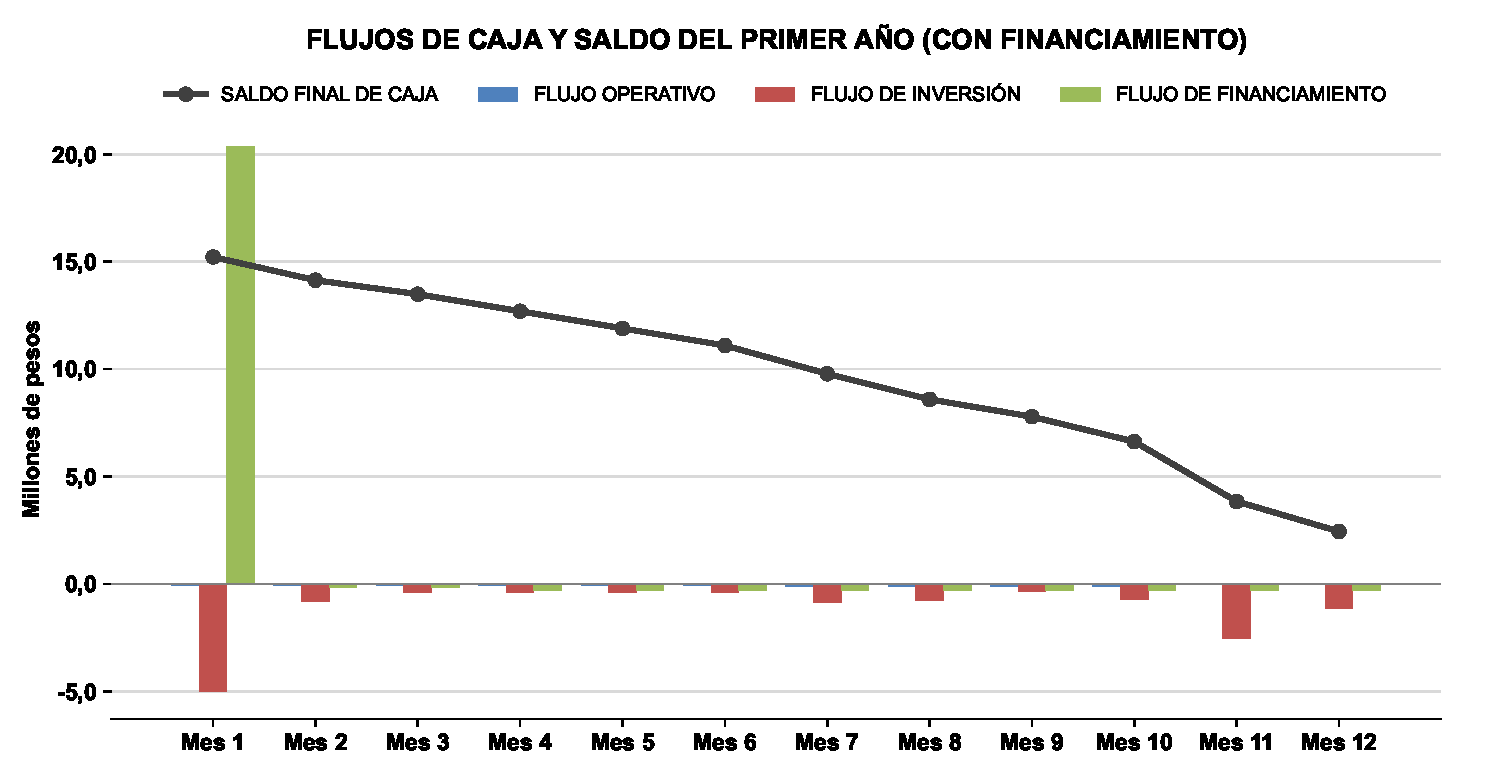
\includegraphics[width=\linewidth]{img/flujo_meses_financiado.pdf}
            \caption{Flujos de caja y saldo del primer año, con financiamiento.}
            \label{fig:flujo_meses_financiado}
        \end{figure}

        \begin{figure}[tbp]
            \centering
            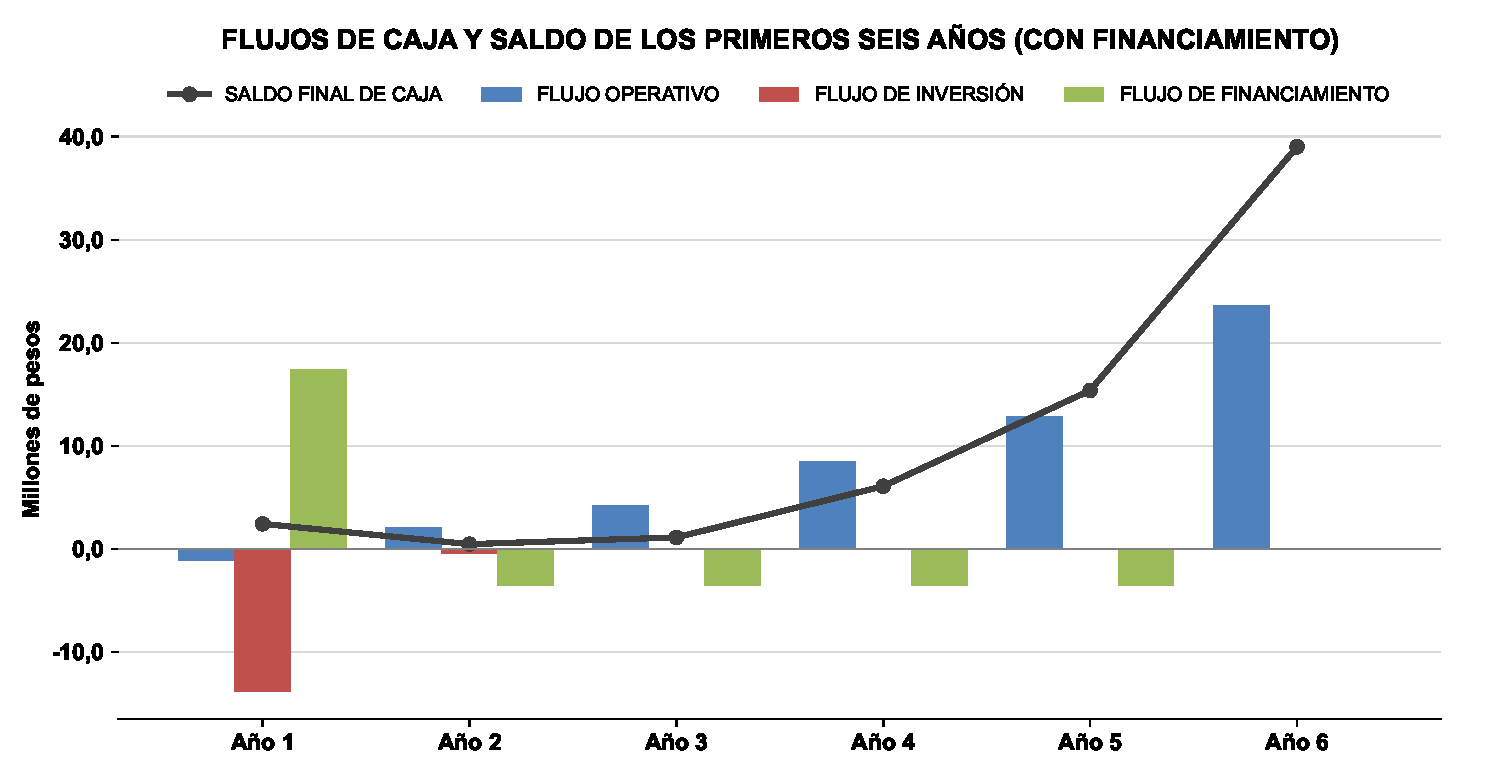
\includegraphics[width=\linewidth]{img/flujo_anios_financiado.pdf}
            \caption{Flujos de caja y saldo de los primeros seis años, con financiamiento.}
            \label{fig:flujo_anios_financiado}
        \end{figure}

        A partir del segundo año la captación crece de manera conservadora: dos suscriptores en el año 2 y tres en el año 3 (clínicas cabecera de Posadas, Oberá y Eldorado), cinco y siete en los años 4 y 5, y doce en el año 6, ya con alcance nacional. La Tabla~\ref{tabla:flujo_anual} resume el flujo de los seis años, y su apertura por rubro se presenta en la Tabla~\ref{tabla:anexo_flujo_anual} del Anexo.

        \begingroup \setstretch{1.1}
        \vspace{0.3cm}\noindent\begin{talltblr}[
            caption = Flujo de caja de los primeros seis años con financiamiento,
            label = tabla:flujo_anual
            ]{
                colspec = {Q[l,m,3.4cm] X[r,m] X[r,m] X[r,m] X[r,m] X[r,m] X[r,m]},
                cells = {font=\scriptsize},
                row{1} = {bg=gray!15, font=\scriptsize\bfseries, halign=c},
                row{4,5,9,10,11} = {bg=gray!15, font=\scriptsize\bfseries},
                hlines, vlines,
                rowsep = 2pt, colsep = 3pt
            }

            Concepto & Año 1 & Año 2 & Año 3 & Año 4 & Año 5 & Año 6 \\

            Ingresos por suscripciones & \$\,360.000 & \$\,4.320.000 & \$\,6.480.000 & \$\,10.800.000 & \$\,15.120.000 & \$\,25.920.000 \\
            Egresos operativos & $-$\$\,1.438.252 & $-$\$\,2.279.452 & $-$\$\,2.279.452 & $-$\$\,2.279.452 & $-$\$\,2.279.452 & $-$\$\,2.279.452 \\
            Flujo de caja operativo & $-$\$\,1.078.252 & \$\,2.040.548 & \$\,4.200.548 & \$\,8.520.548 & \$\,12.840.548 & \$\,23.640.548 \\
            Flujo de caja de inversión & $-$\$\,13.872.740 & $-$\$\,464.000 & \$\,0 & \$\,0 & \$\,0 & \$\,0 \\
            Aporte propio & \$\,8.500.000 & \$\,0 & \$\,0 & \$\,0 & \$\,0 & \$\,0 \\
            Desembolso de los créditos & \$\,12.000.000 & \$\,0 & \$\,0 & \$\,0 & \$\,0 & \$\,0 \\
            Cuotas de los créditos & $-$\$\,3.110.556 & $-$\$\,3.547.408 & $-$\$\,3.547.408 & $-$\$\,3.547.408 & $-$\$\,3.547.408 & \$\,0 \\
            Flujo de caja de financiamiento & \$\,17.389.444 & $-$\$\,3.547.408 & $-$\$\,3.547.408 & $-$\$\,3.547.408 & $-$\$\,3.547.408 & \$\,0 \\
            Flujo de caja neto & \$\,2.438.452 & $-$\$\,1.970.860 & \$\,653.140 & \$\,4.973.140 & \$\,9.293.140 & \$\,23.640.548 \\
            Saldo final de caja & \$\,2.438.452 & \$\,467.591 & \$\,1.120.731 & \$\,6.093.871 & \$\,15.387.010 & \$\,39.027.558 \\

        \end{talltblr}\par\vspace{0.3cm}
        \endgroup

        El momento más exigente es el final del segundo año: los dos suscriptores cubren los costos operativos, pero no las cuotas. Sin aporte propio, la caja acumulada llegaría a $-$\$\,8.032.409 en el mes 24. Por eso el aporte se fija en \$\,8.500.000, de modo que el saldo mínimo resulte positivo (\$\,467.591) y la caja no quede negativa en ningún mes. Desde el tercer año el flujo neto es positivo y el saldo crece hasta \$\,39.027.558 al cierre del sexto año.

        \noindent\colorbox{yellow!10}{%
            \parbox{\dimexpr\linewidth-2\fboxsep}{%
                El flujo original sin financiamiento, previo a estos ajustes, se conserva en las Figuras~\ref{fig:anexo_caja_desarrollo} y~\ref{fig:anexo_caja_años} del Anexo. Las correcciones realizadas sobre aquel modelo se detallan en la hoja Correcciones del archivo de cálculo que acompaña al informe.
            }%
        }
        

    \phantomsection
    \subsection{Precio final del servicio}

        El precio se define a partir de los costos y de la competencia. Los costos fijos anuales de los años 2 a 6 suman \$\,2.279.452 (servidor, herramientas y monotributo). Si además se recupera la inversión pre-operativa en cinco años (\$\,2.774.548 por año), el costo total anual asciende a \$\,5.054.000. Con un promedio de 5,8 suscriptores entre los años 2 y 6, el costo por suscriptor es de unos \$\,72.615 mensuales.

        Sobre esa base, el precio final se fija en \textbf{\$\,180.000 mensuales}, lo que implica un margen de beneficio del 148\,\% sobre el costo unitario. Como los integrantes facturan como monotributistas, el precio no discrimina IVA. Frente a la competencia, equivale a unos 39 informes de Entelai ($\approx$\,\$\,4.586 por informe con IVA), y evita la inversión de USD 20.000 a 40.000 que exige un equipo con \textit{software} propietario. La Tabla~\ref{tabla:precio} resume el cálculo y el punto de equilibrio, calculado según la Ecuación~\ref{eq:pe}:

        \begin{equation}
            Q_e = \frac{CF}{PV - CV_u}
            \label{eq:pe}
        \end{equation}

        \vspace{-0.4 cm}
        \begingroup \setstretch{1.1}
        \vspace{0.3cm}\noindent\begin{talltblr}[
            caption = Determinación del precio final y punto de equilibrio,
            label = tabla:precio
            ]{
                colspec = {X[l,m] Q[r,m,3.6cm]},
                cells = {font=\small},
                row{1} = {bg=gray!15, font=\small\bfseries, halign=c},
                row{6} = {bg=gray!15, font=\small\bfseries},
                hlines, vlines,
                rowsep = 3pt, colsep = 5pt
            }

            Concepto & Valor \\

            Costos fijos anuales, años 2 a 6 ($CF$) & \$\,2.279.452 \\
            Recupero anual de la inversión pre-operativa (5 años) & \$\,2.774.548 \\
            Costo total anual & \$\,5.054.000 \\
            Costo mensual por suscriptor (5,8 suscriptores en promedio) & \$\,72.615 \\
            Precio final de la suscripción mensual & \$\,180.000 \\
            Precio anual por suscriptor ($PV$) & \$\,2.160.000 \\
            Costo variable por suscriptor ($CV_u$) & $\approx$\,\$\,0 \\
            Punto de equilibrio sin las cuotas del crédito & 1,06 $\rightarrow$ 2 suscriptores \\
            Punto de equilibrio con las cuotas del crédito (\$\,5.826.860 anuales) & 2,70 $\rightarrow$ 3 suscriptores \\

        \end{talltblr}\par\vspace{0.3cm}
        \endgroup

        El precio originalmente previsto de \$\,150.000 resultaba insuficiente: con él, la TIR (18,3\,\%) quedaba por debajo de la TREMA una vez incorporados los costos recurrentes de los años 2 a 6 y el monotributo de los integrantes.

    \phantomsection
    \subsection{Tasa de rendimiento mínima aceptable (TREMA)}

        La TREMA es la rentabilidad mínima que exige un inversor para aceptar el proyecto, es decir, su costo de oportunidad (Ecuación~\ref{eq:trema}).

        \begin{equation}
            TREMA = \text{Tasa libre de riesgo} + \text{Prima de riesgo} + \text{Otros}
            \label{eq:trema}
        \end{equation}

        \vspace{-0.4 cm}
        \begingroup \setstretch{1.1}
        \vspace{0.3cm}\noindent\begin{talltblr}[
            caption = Componentes de la TREMA,
            label = tabla:trema
            ]{
                colspec = {Q[l,m,3.6cm] Q[c,m,1.6cm] X[l,m]},
                cells = {font=\small},
                row{1} = {bg=gray!15, font=\small\bfseries, halign=c},
                row{6} = {bg=gray!15, font=\small\bfseries},
                hlines, vlines,
                rowsep = 3pt, colsep = 5pt
            }

            Componente & Valor & Justificación \\

            Tasa libre de riesgo & 4,99\,\% & Rendimiento del bono del Tesoro de EE.UU. a 10 años al 23 de octubre de 2026~\cite{us10y}. \\

            Riesgo país & 7,07\,\% & Índice EMBI de Argentina, 707 puntos básicos al 23 de octubre de 2026~\cite{riesgo_pais}. \\

            Prima de riesgo del proyecto & 10,00\,\% & Emprendimiento sin facturación, que depende de la inscripción ante la ANMAT y de la adopción por parte de los oftalmólogos, en un mercado inicial reducido. \\

            Inflación esperada & No se suma & Los flujos están a precios constantes; sumar la inflación esperada (21,1\,\%~\cite{rem_bcra}) penalizaría dos veces el proyecto. \\

            TREMA & 22,06\,\% & Se redondea a 22,1\,\% en el texto. \\

        \end{talltblr}\par\vspace{0.3cm}
        \endgroup

        Como referencia, la TREMA supera holgadamente el costo de los créditos (15\,\% nominal, negativo en términos reales), por lo que endeudarse para financiar el proyecto es conveniente si este rinde por encima de la TREMA.

    \phantomsection
    \subsection{Valor actual neto (VAN)}

        El VAN descuenta los flujos futuros a la TREMA y les resta la inversión inicial (Ecuación~\ref{eq:van}). Se calcula para el proyecto, sin considerar cómo se financia, y para el inversionista, cuyo flujo incluye el desembolso de los créditos y el pago de las cuotas. La inversión inicial ($I_0$) es la inversión pre-operativa del primer año, de \$\,13.872.740.

        \begin{equation}
            VAN = \sum_{t=1}^{n}\frac{F_{t}}{(1+r)^{t}} - I_{0}
            \label{eq:van}
        \end{equation}

        \vspace{-0.4 cm}
        \begingroup \setstretch{1.1}
        \vspace{0.3cm}\noindent\begin{talltblr}[
            caption = Cálculo del VAN del proyecto y del inversionista (TREMA del 22{,}06\,\%),
            label = tabla:van
            ]{
                colspec = {Q[c,m,1cm] X[r,m] Q[c,m,1.6cm] X[r,m] X[r,m] X[r,m]},
                cells = {font=\small},
                row{1} = {bg=gray!15, font=\small\bfseries, halign=c},
                row{9} = {bg=gray!15, font=\small\bfseries},
                hlines, vlines,
                rowsep = 3pt, colsep = 4pt
            }

            Año ($t$) & Flujo del proyecto & $1/(1+r)^t$ & Flujo descontado & Flujo del inversionista & Flujo descontado \\

            0 & $-$\$\,13.872.740 & 1,0000 & $-$\$\,13.872.740 & $-$\$\,1.872.740 & $-$\$\,1.872.740 \\
            1 & $-$\$\,1.078.252 & 0,8193 & $-$\$\,883.379 & $-$\$\,4.188.808 & $-$\$\,3.431.762 \\
            2 & \$\,1.576.548 & 0,6712 & \$\,1.058.182 & $-$\$\,1.970.860 & $-$\$\,1.322.845 \\
            3 & \$\,4.200.548 & 0,5499 & \$\,2.309.861 & \$\,653.140 & \$\,359.158 \\
            4 & \$\,8.520.548 & 0,4505 & \$\,3.838.611 & \$\,4.973.140 & \$\,2.240.460 \\
            5 & \$\,12.840.548 & 0,3691 & \$\,4.739.327 & \$\,9.293.140 & \$\,3.430.012 \\
            6 & \$\,23.640.548 & 0,3024 & \$\,7.148.540 & \$\,23.640.548 & \$\,7.148.540 \\
            \SetCell[c=3]{r} VAN & & & \$\,4.338.402 & & \$\,6.550.823 \\

        \end{talltblr}\par\vspace{0.3cm}
        \endgroup

        El \textbf{VAN del proyecto es de \$\,4.338.402}. Al ser positivo, los flujos descontados superan la inversión inicial: el proyecto recupera lo invertido, paga la rentabilidad mínima exigida y genera un valor adicional. El VAN del inversionista es mayor (\$\,6.550.823), porque parte de la inversión se financia con deuda a una tasa inferior a la TREMA. Los tres primeros flujos negativos del inversionista ($-$\$\,8.032.409 acumulados) son los que cubre el aporte propio.

    \phantomsection
    \subsection{Tasa interna de retorno (TIR)}

        La TIR es la tasa de descuento que hace que el VAN sea igual a cero (Ecuación~\ref{eq:tir}), y representa la rentabilidad anual propia del proyecto.

        \begin{equation}
            0 = \sum_{t=1}^{n}\frac{F_{t}}{(1+TIR)^{t}} - I_{0}
            \label{eq:tir}
        \end{equation}

        La Tabla~\ref{tabla:indicadores} resume los indicadores. La \textbf{TIR del proyecto es del 29,0\,\%}, superior a la TREMA del 22,1\,\%, y la del inversionista alcanza el 42,8\,\%. Además, la inversión se recupera en 4,05 años sin descontar y en 5,39 años con los flujos descontados, en ambos casos dentro del horizonte de evaluación.

        \begingroup \setstretch{1.1}
        \vspace{0.3cm}\noindent\begin{talltblr}[
            caption = Indicadores de evaluación económica y financiera,
            label = tabla:indicadores
            ]{
                colspec = {X[l,m] Q[r,m,3.2cm] Q[r,m,3.2cm]},
                cells = {font=\small},
                row{1} = {bg=gray!15, font=\small\bfseries, halign=c},
                hlines, vlines,
                rowsep = 3pt, colsep = 5pt
            }

            Indicador & Proyecto & Inversionista \\

            TREMA & 22,1\,\% & 22,1\,\% \\
            Valor actual neto (VAN) & \$\,4.338.402 & \$\,6.550.823 \\
            Tasa interna de retorno (TIR) & 29,0\,\% & 42,8\,\% \\
            Período de recupero simple & 4,05 años & --- \\
            Período de recupero descontado & 5,39 años & --- \\
            Criterio de la guía (TIR $>$ TREMA y VAN $>$ 0) & Se cumple & Se cumple \\

        \end{talltblr}\par\vspace{0.3cm}
        \endgroup

    \phantomsection
    \subsection{Análisis de sensibilidad}

        La Tabla~\ref{tabla:sensibilidad} muestra cómo varían los indicadores al modificar un parámetro por vez. La última columna indica el aporte que haría falta en cada escenario para que la caja no quede negativa.

        \begingroup \setstretch{1.1}
        \vspace{0.3cm}\noindent\begin{talltblr}[
            caption = Análisis de sensibilidad del proyecto,
            label = tabla:sensibilidad
            ]{
                colspec = {X[l,m] Q[r,m,2.3cm] Q[c,m,1.4cm] Q[r,m,2.3cm] Q[c,m,1.5cm] Q[r,m,2.3cm]},
                cells = {font=\footnotesize},
                row{1} = {bg=gray!15, font=\footnotesize\bfseries, halign=c},
                row{2} = {bg=gray!15},
                hlines, vlines,
                rowsep = 3pt, colsep = 4pt
            }

            Escenario & VAN del proyecto & TIR del proyecto & VAN del inversionista & TIR del inversionista & Mínimo de caja sin aporte \\

            Caso base & \$\,4.338.402 & 29,0\,\% & \$\,6.550.823 & 42,8\,\% & $-$\$\,8.032.409 \\
            Precio de \$\,150.000 ($-$17\,\%) & \$\,164.761 & 22,3\,\% & \$\,2.377.182 & 30,0\,\% & $-$\$\,9.239.269 \\
            Precio de \$\,210.000 (+17\,\%) & \$\,8.512.043 & 34,9\,\% & \$\,10.724.464 & 54,4\,\% & $-$\$\,7.252.409 \\
            Un suscriptor menos por año & $-$\$\,722.661 & 20,9\,\% & \$\,1.489.760 & 26,6\,\% & $-$\$\,11.699.269 \\
            Costos +20\,\% & \$\,197.713 & 22,3\,\% & \$\,2.410.134 & 27,8\,\% & $-$\$\,11.643.298 \\
            Lanzamiento demorado 6 meses & $-$\$\,1.161.805 & 20,1\,\% & \$\,1.050.616 & 25,5\,\% & $-$\$\,10.945.839 \\
            Un solo crédito de \$\,6.000.000 & \$\,4.338.402 & 29,0\,\% & \$\,5.444.612 & 33,4\,\% & $-$\$\,10.725.664 \\
            TREMA del 17,1\,\% (prima del 5\,\%) & \$\,8.542.416 & 29,0\,\% & \$\,9.581.851 & 42,8\,\% & $-$\$\,8.032.409 \\
            TREMA del 27,1\,\% (prima del 15\,\%) & \$\,1.067.755 & 29,0\,\% & \$\,4.260.731 & 42,8\,\% & $-$\$\,8.032.409 \\
            Consultoría oftalmológica completa (sin convenio) & \$\,1.758.402 & 24,6\,\% & \$\,3.970.823 & 31,8\,\% & $-$\$\,10.612.409 \\

        \end{talltblr}\par\vspace{0.3cm}
        \endgroup

        Los parámetros más sensibles son la demanda y los plazos. Con un suscriptor menos por año o con un lanzamiento demorado seis meses, el VAN del proyecto se vuelve negativo, aunque el del inversionista se mantiene positivo gracias al apalancamiento. Bajar el precio a \$\,150.000 o aumentar los costos un 20\,\% deja al proyecto en el límite de la TREMA. Si se aprobara un solo crédito, la rentabilidad seguiría siendo aceptable, pero el aporte propio necesario subiría a unos \$\,11.000.000.

    \phantomsection
    \subsection{¿Es atractivo para el inversionista?}

        Sí, aunque con condiciones. KERALYTIX resulta rentable para el inversionista dando un TIR del proyecto (29,0\,\%) supera la TREMA (22,1\,\%) y el VAN es positivo (\$\,4.338.402). El atractivo se apoya además en:

        \begin{itemize}
            \item \textbf{Apalancamiento favorable:} los créditos cuestan un 15\,\% fijo, por debajo de la TREMA y negativo en términos reales, lo que eleva la TIR del inversionista al 42,8\,\%.

            \item \textbf{Escalabilidad:} el costo de atender a un suscriptor adicional es prácticamente nulo, por lo que el flujo crece casi en la misma proporción que las suscripciones.

            \item \textbf{Ventaja competitiva:} no hay competidores nacionales con un producto específico para queratocono, y la inscripción ante la ANMAT constituye una barrera de entrada para nuevos competidores.

            \item \textbf{Beneficio para el sistema de salud:} una detección temprana puede evitar tratamientos que cuestan entre veinte y más de sesenta veces lo que un estudio topográfico (ver Impacto económico).
        \end{itemize}

        Sin embargo, el margen sobre la TREMA es moderado y depende del ritmo de captación: una demora de seis meses o un suscriptor menos por año vuelven negativo el VAN del proyecto. Por eso KERALYTIX resulta atractivo para un inversor que acepte el riesgo de una etapa temprana, siempre que se cumplan las condiciones de financiamiento que se detallan a continuación.

    \phantomsection
    \subsection{Consideraciones sobre el esquema de financiamiento}

        La viabilidad calculada depende de las siguientes condiciones, que deben confirmarse con un oficial de crédito del FCM antes de iniciar el trámite:

        \begin{itemize}
            \item \textbf{Dos créditos para un mismo proyecto:} el tope de \$\,6.000.000 es por solicitante, y cada pedido requiere su propio formulario, presupuestos, localización y habilitación. El FCM podría considerar ambos pedidos como un único emprendimiento y aprobar solo uno (R9).

            \item \textbf{Tasa sujeta a la TAMAR:} la tasa es el 60\,\% de la TAMAR vigente al firmar el contrato. Si la TAMAR sube antes de la firma, la cuota aumenta.

            \item \textbf{Gastos de otorgamiento:} los costos de escribanía, seguros, tasación (si hay hipoteca) e inscripción de la prenda no están incluidos en el flujo.

            \item \textbf{Destino de los fondos:} los honorarios solo son financiables si el FCM los acepta como investigación y desarrollo, y la porción de capital de trabajo debe devolverse en doce meses (R11). Si no se aceptan, el crédito se reduce a los rubros admitidos y la diferencia se cubre con aporte propio.

            \item \textbf{Garantes y bienes de terceros:} cada crédito necesita su garantía. Un garante debe acreditar ingresos de al menos 5 veces la cuota, y un vehículo o inmueble familiar queda comprometido hasta cancelar el crédito.

            \item \textbf{Monotributo e Ingresos Brutos:} cada integrante debe inscribirse antes de firmar. Con 12 suscriptores, los ingresos del año 6 (\$\,12.960.000 por integrante) superan el tope anual de la categoría A (\$\,12.009.410~\cite{monotributo_2026}), por lo que será necesario recategorizarse o constituir una sociedad.

            \item \textbf{Localización:} se debe acreditar el lugar del emprendimiento, por ejemplo, mediante un comodato con la UNaM o con una incubadora del Parque Tecnológico Misiones.

            \item \textbf{Aporte propio:} los \$\,8.500.000 superan ampliamente el capital inicial de los integrantes, por lo que dependen de ahorros y aportes familiares. Es la condición principal para que la caja no quede negativa en el segundo año.

            \item \textbf{Fuentes de la información:} las condiciones del FCM se tomaron de sus preguntas frecuentes, infografías y notas de prensa de 2026, y pueden modificarse.
        \end{itemize}


    % Conclusiones y líneas futuras
    \phantomsection
\chapter{Conclusiones}

    % Pendiente: conclusiones del trabajo

\phantomsection
\section{Líneas futuras}
\label{sec:lineas_futuras}

    Quedan fuera del alcance del PFI, y se plantean como líneas futuras, los siguientes puntos.

    \begin{itemize}
        \item La estratificación del riesgo, ya sea con los índices del sistema ABCD de Belin o con la predicción del riesgo de progresión mediante redes neuronales recurrentes. Ambas necesitan datos que CornOrb no incluye, como los valores ABCD o estudios de un mismo paciente en distintas visitas.

        \item La validación clínica con muestras locales de distintos centros de salud de la región, a partir de las solicitudes ya iniciadas (ver capítulo Desarrollo).

        \item La adaptación de modelos fundacionales al análisis de la topografía corneal. Requiere conjuntos de datos del segmento anterior del ojo y una capacidad de cómputo que exceden el PFI.

        \item La compatibilidad con otros equipos de diagnóstico, como Pentacam\textsuperscript{\scriptsize\textregistered}{} o Sirius\textsuperscript{\scriptsize\textregistered}{}, que depende de obtener sus archivos de exportación.

        \item La inscripción de KERALYTIX como producto médico ante la ANMAT y su lanzamiento comercial, cuya planificación se desarrolla en el capítulo Estudio financiero.
    \end{itemize}


    % Bibliografía
    \clearpage
    \phantomsection
    \renewcommand{\bibname}{Referencias}
    \bibliographystyle{IEEEtran}
    \bibliography{partes/bibliografia}

    % Anexo de imágenes
    % \clearpage
\phantomsection
\chapter{Anexo de imágenes}
\label{chap:anexo_imagenes}

%\section{Imágenes del Proyecto Técnico}

    % Colores del diagrama: PFI, reserva de contingencia y proyección del producto
    \definecolor{ganttpfi}{HTML}{2E86AB}
    \definecolor{ganttreserva}{HTML}{BBBBBB}
    \definecolor{ganttproducto}{HTML}{E4572E}

    \begin{figure}[H] \centering
        \begin{ganttchart}[
                hgrid, vgrid,
                x unit = 0.78cm,
                y unit title = 0.6cm,
                y unit chart = 0.55cm,
                title/.append style = {fill=gray!15},
                title label font = \small\bfseries,
                bar label font = \small,
                group label font = \small\bfseries,
                milestone label font = \small\itshape,
                bar/.append style = {fill=ganttpfi, draw=none},
                bar height = 0.55,
                group/.append style = {fill=black!75},
                group height = 0.25,
                group peaks height = 0.15,
                group peaks width = 0.12,
                group left shift = 0,
                group right shift = 0,
                milestone/.append style = {fill=black!75},
                milestone height = 0.55,
            ]{1}{11}

            \gantttitle{PFI}{6} \gantttitle{Proyección del producto}{5} \\
            \gantttitlelist{1,...,11}{1} \\

            \ganttbar{Documentación y trazabilidad}{1}{10} \\

            \ganttgroup{Fase 1: datos y modelo}{1}{3} \\
            \ganttbar{Requisitos regulatorios}{1}{1} \\
            \ganttbar{Análisis exploratorio de datos}{1}{1} \\
            \ganttbar{Preprocesamiento de los datos}{1}{2} \\
            \ganttbar{Entrenamiento del modelo}{2}{3} \\
            \ganttbar{Evaluación e integración de Grad-CAM}{3}{3} \\
            \ganttbar{Solicitud de muestras locales}{1}{4} \\

            \ganttgroup{Fase 2: aplicación web}{3}{4} \\
            \ganttbar{\textit{Backend} (API con FastAPI)}{3}{4} \\
            \ganttbar{\textit{Frontend} (React)}{3}{4} \\
            \ganttbar{Usuarios y suscripción}{4}{4} \\
            \ganttbar{Despliegue en servidor VPS}{4}{4} \\
            \ganttmilestone{Prototipo terminado}{4} \\

            \ganttbar[bar/.append style={fill=ganttreserva}]{Reserva de contingencia}{5}{6} \\

            \ganttgroup{Fase 3: validación clínica}{7}{8} \\
            \ganttbar[bar/.append style={fill=ganttproducto}]{Evaluación con muestras locales}{7}{8} \\
            \ganttbar[bar/.append style={fill=ganttproducto}]{Pruebas de usabilidad}{8}{8} \\

            \ganttgroup{Fase 4: certificación y lanzamiento}{9}{10} \\
            \ganttbar[bar/.append style={fill=ganttproducto}]{Cierre del informe técnico}{9}{9} \\
            \ganttbar[bar/.append style={fill=ganttproducto}]{Inscripción ante la ANMAT}{9}{10} \\
            \ganttbar[bar/.append style={fill=ganttproducto}]{Documentación legal}{9}{10} \\
            \ganttbar[bar/.append style={fill=ganttproducto}]{Comunicación y manual de usuario}{10}{10} \\
            \ganttmilestone{Lanzamiento comercial}{10}

        \end{ganttchart}
        \caption{Diagrama de Gantt de las actividades del proyecto.}
        \label{fig:anexo_gantt}
    \end{figure}


%\section{Imágenes del Análisis de Producto de Mercado}

    \begin{landscape}
        \thispagestyle{empty}
        \begin{figure}[H] \centering
        
            \makebox[\linewidth][c]{\hspace*{1 cm}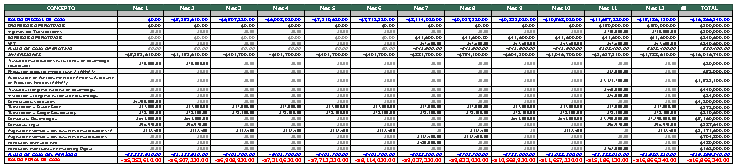
\includegraphics[height=0.39\textheight]{img/caja_desarrollo.pdf}}
            \caption{Flujo de caja correspondiente al desarrollo del proyecto (primer año).}
            \label{fig:anexo_caja_desarrollo}
            
            \makebox[\linewidth][c]{\hspace*{1 cm}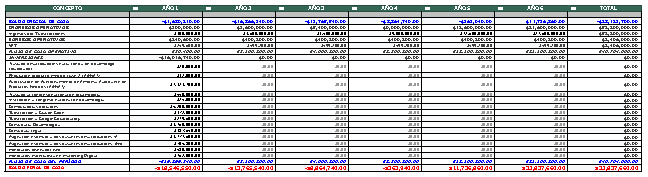
\includegraphics[height=0.45\textheight]{img/caja_años.pdf}}
            \caption{Flujo de caja correspondiente a los primeros seis años.}
            \label{fig:anexo_caja_años}
        \end{figure}
    \end{landscape}


\phantomsection
\section{Anexo del estudio financiero}
\label{sec:anexo_estudio_financiero}

    \subsection*{Criterios de factibilidad}

        \begingroup \setstretch{1.1}
        \begin{longtblr}[
            caption = Criterios ponderados para la evaluación de factibilidad,
            label = tabla:anexo_criterios
            ]{
                colspec = {Q[l,m,2.4cm] Q[c,m,1.4cm] X[l,m]},
                cells = {font=\small},
                row{1} = {bg=gray!15, font=\small\bfseries, halign=c},
                hlines, vlines,
                rowsep = 3pt, colsep = 5pt
            }

            Criterio & Peso & Aspectos evaluados \\

            Técnico & 40\,\% & Determina si el equipo cuenta con los recursos y la experiencia para cumplir los requisitos: accesibilidad de tecnologías y datos (\textit{hardware} de entrenamiento, herramientas y \textit{datasets} multimodales), capacidad técnica del equipo (\textit{Deep Learning}, \textit{backend}, \textit{frontend} y normativa médica), interoperabilidad con distintos equipos (Orbscan, Pentacam o Sirius) y mantenibilidad ante nuevas versiones o cambios en los formatos de salida. \\

            Jurídico & 25\,\% & Asegura el cumplimiento normativo en salud: inscripción como producto médico Clase II ante la ANMAT según las disposiciones N.º 2318/2002~\cite{dispo_2318} y N.º 9688/2019~\cite{dispo_9688}, anonimización de los datos según la Ley N.º 25.326~\cite{ley_25326} y gestión del consentimiento informado de los pacientes. \\

            Operativo & 20\,\% & Analiza si el sistema se utilizará y funcionará al instalarse: predisposición de los oftalmólogos a adoptar herramientas de IA, facilidad de uso para personal con poca experiencia digital e integración al flujo de trabajo de la consulta. \\

            Económico & 15\,\% & Evalúa la rentabilidad y la capacidad de solventar los gastos: costos directos de desarrollo e implementación (Colab Pro, VPS y aranceles de la ANMAT), costos de validación clínica y relación costo-beneficio para los especialistas. \\

        \end{longtblr}
        \endgroup

        \begingroup \setstretch{1.1}
        \begin{longtblr}[
            caption = Análisis de cada criterio de factibilidad,
            label = tabla:anexo_analisis_criterios
            ]{
                colspec = {Q[l,m,2cm] Q[l,m,2.8cm] X[l,m]},
                cells = {font=\small},
                row{1} = {bg=gray!15, font=\small\bfseries, halign=c},
                cell{2}{1} = {r=4}{}, cell{6}{1} = {r=3}{}, cell{9}{1} = {r=3}{}, cell{12}{1} = {r=3}{},
                hlines, vlines,
                rowsep = 3pt, colsep = 5pt
            }

            Criterio & Aspecto & Análisis \\

            Técnico & Tecnologías y datos & Se dispone del \textit{dataset} público y multimodal CornOrb~\cite{zenodo}, cuyo análisis exploratorio confirmó que es adecuado como punto de partida. Las herramientas son de uso libre (Python, FastAPI, React) y el cómputo se obtiene con Google Colab Pro. Las muestras locales están en proceso de solicitud a nueve centros y no condicionan el prototipo. \\
            & Capacidad del equipo & Los integrantes tienen experiencia académica en aprendizaje profundo y aplicaciones web. El conocimiento normativo se complementa con el abogado consultor. \\
            & Interoperabilidad & Es el aspecto más limitado: el prototipo procesa solo mapas de equipos Orbscan. La compatibilidad con Pentacam o Sirius depende de acceder a sus archivos de exportación y queda como trabajo futuro. \\
            & Mantenibilidad & Los módulos independientes (preprocesamiento, modelo, API e interfaz) y los contenedores permiten actualizar cada parte por separado. \\

            Jurídico & Normativa ANMAT & La inscripción como Clase II exige demostrar seguridad y eficacia mediante validación clínica, prevista en la proyección del producto. El prototipo del PFI no se usa para decisiones clínicas, y desde el inicio se lleva la documentación que la inscripción requerirá. \\
            & Datos personales & La Ley N.º 25.326 considera sensibles los datos de salud~\cite{ley_25326}, por lo que todo estudio debe estar anonimizado: los de CornOrb ya lo están, y las muestras locales se anonimizan en su origen. \\
            & Consentimiento informado & Su gestión depende de los centros colaboradores y forma parte de las solicitudes en curso. \\

            Operativo & Aceptación del usuario & Se estima favorable, porque la herramienta responde a una dificultad diagnóstica reconocida y apoya al especialista sin reemplazarlo. La resistencia a la IA es un riesgo identificado (R7). \\
            & Facilidad de uso & Al ser una aplicación web, no requiere instalación. El informe presenta el resultado, la confianza y el mapa de calor, y la interfaz cuenta con un especialista en experiencia de usuario. \\
            & Flujo de trabajo & El oftalmólogo carga los mapas que ya exporta su equipo. El paso adicional en la consulta se evaluará en las pruebas de usabilidad. \\

            Económico & Costos directos & La infraestructura tecnológica tiene un costo mensual acotado; los gastos de mayor peso son la habilitación ante la ANMAT y los recursos humanos. \\
            & Validación clínica & Los honorarios del oftalmólogo consultor son uno de los ítems más costosos; la mitad de las horas se cubre por convenio académico. \\
            & Costo-beneficio & Los tratamientos de etapas avanzadas cuestan entre veinte y más de sesenta veces un estudio topográfico. Para el proyecto, la viabilidad depende de financiar la inversión inicial hasta que las suscripciones generen ingresos (ver sección Viabilidad económica y financiera). \\

        \end{longtblr}
        \endgroup

    \subsection*{Presupuesto detallado}

        \begingroup \setstretch{1.1}
        \begin{longtblr}[
            caption = Recursos materiales del proyecto,
            label = tabla:anexo_recursos_materiales
            ]{
                colspec = {Q[l,m,3.4cm] X[l,m] Q[r,m,2.6cm]},
                cells = {font=\small},
                row{1} = {bg=gray!15, font=\small\bfseries, halign=c},
                row{5} = {bg=gray!15, font=\small\bfseries},
                hlines, vlines,
                rowsep = 3pt, colsep = 5pt
            }

            Recurso & Descripción & Costo \\

            Muestras locales & Lote de 150 topografías corneales anonimizadas, provistas por el consultorio asociado para la validación clínica local. & \$\,0,00 \\

            \textit{Datasets} públicos & Bases de datos internacionales con casos de queratocono para el entrenamiento inicial del modelo. & \$\,0,00 \\

            Computadoras portátiles & Dos equipos con procesador Intel Core i7 y 16 GB de RAM, uno por integrante, a \$\,2.100.000 cada uno. & \$\,4.200.000,00 \\

            \SetCell[c=2]{r} TOTAL & & \$\,4.200.000,00 \\

        \end{longtblr}
        \endgroup

        \begingroup \setstretch{1.1}
        \begin{longtblr}[
            caption = Recursos humanos propios que intervendrán en el proyecto,
            label = tabla:rrhh_propios
            ]{
                colspec = {X[l,m] Q[c,m,1cm] Q[r,m,2.3cm] Q[r,m,2.1cm] Q[c,m,1.4cm] Q[c,m,1.2cm] Q[r,m,2.3cm]},
                cells = {font=\footnotesize},
                row{1} = {bg=gray!15, font=\footnotesize\bfseries, halign=c},
                row{4} = {bg=gray!15, font=\footnotesize\bfseries},
                hlines, vlines,
                rowsep = 3pt, colsep = 3pt
            }

            Profesión / función en el proyecto & Cant. & Costo mensual real c/u & Retribución simbólica & Meses de partic. & \% de dedic. & Costo total \\

            Programador IA & 2 & \$\,3.783.577,52 & \$\,352.400,00 & 9 & 50 & \$\,3.171.600,00 \\

            Desarrollador Web Full Stack & 2 & \$\,3.453.169,23 & \$\,352.400,00 & 2 & 50 & \$\,704.800,00 \\

            \SetCell[c=6]{r} TOTAL & & & & & & \$\,3.876.400,00 \\

        \end{longtblr}
        \endgroup

        Los costos mensuales reales se basan en los honorarios recomendados por el Consejo Profesional de Ciencias Informáticas de Córdoba~\cite{honorarios_profesionales_cordoba}, y la retribución simbólica en el Salario Mínimo, Vital y Móvil~\cite{cita:SMVM}, en proporción a una jornada de cuatro horas. Los recursos humanos adicionales se valúan según el salario mediano de cada rol~\cite{cita:salario_marketing,cita:salario_UX_UI}.

        \begingroup \setstretch{1.1}
        \begin{longtblr}[
            caption = Recursos humanos adicionales requeridos en el proyecto,
            label = tabla:rrhh_adicionales
            ]{
                colspec = {Q[l,m,2.4cm] X[l,m] Q[r,m,2.5cm] Q[c,m,1.5cm] Q[c,m,1.4cm] Q[r,m,2.3cm]},
                cells = {font=\small},
                row{1} = {bg=gray!15, font=\small\bfseries, halign=c},
                row{4,5} = {bg=gray!15, font=\small\bfseries},
                hlines, vlines,
                rowsep = 3pt, colsep = 5pt
            }

            Profesión u oficio & Función en el proyecto & Costo total mensual & Meses de partic. & \% de dedic. & Costo total \\

            Diseñador web & Diseño de las interfaces UI/UX & \$\,1.600.000,00 & 1 & 30 & \$\,480.000,00 \\

            Idóneo & Marketing digital & \$\,810.000,00 & 1 & 20 & \$\,162.000,00 \\

            \SetCell[c=5]{r} TOTAL & & & & & \$\,642.000,00 \\

            \SetCell[c=5]{r} TOTAL DE RECURSOS HUMANOS & & & & & \$\,4.518.400,00 \\

        \end{longtblr}
        \endgroup

        \begingroup \setstretch{1.1}
        \begin{longtblr}[
            caption = Consultoría y servicios tecnológicos a contratar,
            label = tabla:consultoria_servicios
            ]{
                colspec = {X[l,m] Q[r,m,2.8cm] Q[c,m,2.6cm] Q[r,m,2.8cm]},
                cells = {font=\small},
                row{1} = {bg=gray!15, font=\small\bfseries, halign=c},
                row{6} = {bg=gray!15, font=\small\bfseries},
                hlines, vlines,
                rowsep = 3pt, colsep = 5pt
            }

            Descripción & Costo mensual & Meses de partic. & Costo total \\

            Google Colaboratory (Pro) & \$\,18.300,00 & 12 & \$\,219.600,00 \\

            Suscripción a Claude Code & \$\,31.000,00 & 12 & \$\,372.000,00 \\

            Abogado - Consultor & \$\,96.910,00 & 4 & \$\,387.640,00 \\

            Lic. en Oftalmología - Consultor (20 h pagas de 40) & \$\,860.000,00 & 3 & \$\,2.580.000,00 \\

            \SetCell[c=3]{r} TOTAL & & & \$\,3.559.240,00 \\

        \end{longtblr}
        \endgroup

        La hora médica del oftalmólogo se valúa en \$\,129.000 según el Colegio de Médicos de Misiones~\cite{cita:honorario_oftalmólogo}, y la consultoría legal según los valores del Colegio de Abogados de Misiones~\cite{cita:honorario_abogado}. El servidor VPS (\$\,41.600 mensuales desde el mes 7) se contabiliza como costo operativo.

        \begingroup \setstretch{1.1}
        \begin{longtblr}[
            caption = {Costos de movilidad, logística, inscripción a congresos y matriculación},
            label = tabla:otros_costos
            ]{
                colspec = {X[l,m] Q[c,m,1.6cm] Q[r,m,3cm]},
                cells = {font=\small},
                row{1} = {bg=gray!15, font=\small\bfseries, halign=c},
                row{7} = {bg=gray!15, font=\small\bfseries},
                hlines, vlines,
                rowsep = 3pt, colsep = 5pt
            }

            Descripción & Período & Costo total \\

            Traslados de los desarrolladores a la clínica del oftalmólogo colaborador (Oberá / Leandro N. Alem) & Meses 1 y 2 & \$\,20.000,00 \\

            Registro de producto médico Clase II - ANMAT & Mes 11 & \$\,52.000,00 \\

            Autorización de funcionamiento de empresa fabricante de productos médicos - ANMAT & Mes 11 & \$\,1.523.100,00 \\

            Traslado al congreso nacional de oftalmología (Oberá / Buenos Aires) & Año 2 & \$\,440.000,00 \\

            Inscripción al congreso nacional de oftalmología~\cite{cita:aranceles_congreso_oftalmología} & Año 2 & \$\,24.000,00 \\

            \SetCell[c=2]{r} TOTAL & & \$\,2.059.100,00 \\

        \end{longtblr}
        \endgroup

    \subsection*{Criterios y planes de la gestión de riesgos}

        \begingroup \setstretch{1.1}
        \begin{longtblr}[
            caption = Escala de probabilidad de ocurrencia de riesgos,
            label = riesgos_prob
            ]{
                colspec = {Q[c,m,2.5cm] Q[c,m,2.5cm] X[l,m]},
                cells = {font=\small},
                row{1} = {bg=gray!15, font=\small\bfseries, halign=c},
                hlines, vlines,
                rowsep = 3pt, colsep = 5pt
            }

            Cualitativa & Cuantitativa & Descripción \\
            Recurrente  & 5 & Este riesgo ocurrirá en algún momento \\
            Probable    & 4 & Existe una gran probabilidad de que este riesgo ocurra \\
            Posible     & 3 & Este riesgo podría ocurrir o no, probabilidades de 50/50 \\
            Inusual     & 2 & Existe una gran probabilidad de que este riesgo no ocurra \\
            Remota      & 1 & El hecho de que este riesgo ocurra es una posibilidad remota \\

        \end{longtblr}
        \endgroup

        \begingroup \setstretch{1.1}
        \begin{longtblr}[
            caption = Escala de gravedad de ocurrencia de riesgos,
            label = riesgos_grav
            ]{
                colspec = {Q[c,m,2.5cm] Q[c,m,2.5cm] X[l,m]},
                cells = {font=\small},
                row{1} = {bg=gray!15, font=\small\bfseries, halign=c},
                hlines, vlines,
                rowsep = 3pt, colsep = 5pt
            }

            Cualitativa & Cuantitativa & Descripción \\
            Catastrófica & 5 & Las consecuencias de este riesgo serán muy perjudiciales y puede resultar difícil recuperarse \\
            Importante & 4 & Las consecuencias de este riesgo serán significativas y pueden causar daños a largo plazo \\
            Moderada & 3 & Las consecuencias del riesgo tardarán en mitigarse \\
            Menor & 2 & Las consecuencias del riesgo se gestionarán con facilidad \\
            Insignificante & 1 & El riesgo generará pocas consecuencias si ocurriera \\

        \end{longtblr}
        \endgroup

        \begingroup \setstretch{1.1}
        \begin{longtblr}[
            caption = Escala de impacto de riesgos considerando probabilidad y gravedad,
            label = riesgos_imp
            ]{
                colspec = {X[c,m] X[c,m] X[c,m] X[c,m] X[c,m] X[c,m]},
                cells = {font=\small},
                row{1} = {bg=gray!15, font=\small\bfseries, halign=c},
                column{1} = {bg=gray!15, font=\small\bfseries},
                cell{2}{2,3,4} = {bg=red!25}, cell{2}{5} = {bg=orange!30}, cell{2}{6} = {bg=green!25},
                cell{3}{2,3} = {bg=red!25}, cell{3}{4,5} = {bg=orange!30}, cell{3}{6} = {bg=green!25},
                cell{4}{2} = {bg=red!25}, cell{4}{3,4} = {bg=orange!30}, cell{4}{5,6} = {bg=green!25},
                cell{5}{2,3} = {bg=orange!30}, cell{5}{4,5,6} = {bg=green!25},
                cell{6}{2,3,4,5,6} = {bg=green!25},
                hlines, vlines,
                rowsep = 3pt, colsep = 5pt
            }

                        & Catastrófica & Importante & Moderada & Menor & Insignificante \\
            Recurrente  & 25 & 20 & 15 & 10 & 5 \\
            Probable    & 20 & 16 & 12 & 8  & 4 \\
            Posible     & 15 & 12 & 9  & 6  & 3 \\
            Inusual     & 10 & 8  & 6  & 4  & 2 \\
            Remota      & 5  & 4  & 3  & 2  & 1 \\

        \end{longtblr}
        \endgroup

        \begingroup \setstretch{1.1}
        \begin{longtblr}[
            caption = Descripción y planes de acción de los riesgos identificados,
            label = tabla:anexo_planes_riesgos
            ]{
                colspec = {Q[c,m,0.9cm] X[l,m] X[l,m] X[l,m]},
                cells = {font=\footnotesize},
                row{1} = {bg=gray!15, font=\footnotesize\bfseries, halign=c},
                hlines, vlines,
                rowsep = 3pt, colsep = 4pt
            }

            ID & Descripción & Mitigación & Contingencia \\

            R1 & El modelo podría perder eficacia con topografías de pacientes locales, porque se entrena con \textit{datasets} internacionales, y generar falsos negativos. & \textit{Data augmentation} sobre las muestras locales, control del \textit{overfitting} y del \textit{underfitting}, reentrenamiento continuo y monitoreo de deriva. & Sesiones con el oftalmólogo consultor para analizar los mapas de calor de los casos erróneos y reentrenar el modelo de forma focalizada. \\

            R2 & Los equipos de las clínicas podrían exportar formatos propietarios, anómalos o con resoluciones que el preprocesamiento no interprete. & Solicitar muestras de los equipos locales (Pentacam) desde el inicio y construir un \textit{pipeline} de preprocesamiento robusto. & Forzar una estandarización (recorte, redimensionamiento y normalización de canales) antes de que la imagen ingrese al modelo. \\

            R3 & Dificultad para obtener las muestras locales a tiempo, por falta de tiempo de los médicos o trabas en la anonimización. & Entregar a los colaboradores un \textit{script} que elimine automáticamente los metadatos del paciente. & Ampliar la solicitud a otras clínicas de Posadas, Oberá y Eldorado. \\

            R4 & Errores o incompatibilidades al integrar el modelo (Python) con la interfaz (React) y montarlos en el VPS. & Desarrollo modular, probando los \textit{endpoints} de la API antes de conectarlos a la interfaz. & Contenerización con Docker para garantizar el mismo entorno en desarrollo y en el servidor. \\

            R5 & El presupuesto podría superarse por aumentos en los servicios en la nube, los honorarios o los aranceles regulatorios. & Control de gastos, uso de Colab Pro solo en períodos críticos y convenio académico con el oftalmólogo, que ofrece coautoría a cambio de la mitad de las horas. & Asociación con una institución ya habilitada ante la ANMAT o distribución inicial como \textit{software} de investigación (\textit{Research Use Only}). \\

            R6 & Retrasos burocráticos en la inscripción y la auditoría, que postergan el uso clínico formal sin detener el desarrollo. & Sin plan específico por tratarse de un riesgo bajo; la documentación y la trazabilidad se llevan desde el inicio del desarrollo. & --- \\

            R7 & Desconfianza de algunos oftalmólogos y técnicos para incorporar la IA como segunda opinión. & Sin plan específico por tratarse de un riesgo bajo; la aceptación se confirma en las pruebas con usuarios. & --- \\

            R8 & Desacuerdos técnicos o de disponibilidad entre los integrantes que ralenticen ciertas tareas. & Sin plan específico por tratarse de un riesgo bajo. & --- \\

            R9 & El FCM podría considerar los dos pedidos como un único emprendimiento y aprobar solo un crédito, o un monto menor. & Consultar a un oficial de crédito antes de presentar, y presentar cada solicitud con un destino diferenciado (modelo de IA y plataforma web) y documentación propia. & Cubrir la diferencia con aporte propio adicional (unos \$\,2.700.000 más), comprar una sola computadora o postular a premios y subsidios para emprendedores. \\

            R10 & Si el lanzamiento o la captación se demoran, las cuotas siguen venciendo sin ingresos suficientes y la deuda recae sobre los garantes o los bienes ofrecidos. & Dimensionar el aporte propio con margen sobre el peor mes de caja, tomar la tasa fija y sumar al oftalmólogo colaborador como primer suscriptor. & Solicitar la refinanciación al FCM, postergar los gastos no esenciales y ofrecer descuentos por pago anual para adelantar ingresos. \\

            R11 & El FCM podría no aceptar los honorarios como investigación y desarrollo, o exigir la devolución del capital de trabajo en doce meses. & Presentar presupuestos solo de rubros financiables y confirmar la excepción de investigación y desarrollo antes de firmar. & Reducir el monto solicitado a los rubros admitidos y cubrir el resto con aporte propio. \\

        \end{longtblr}
        \endgroup

    \subsection*{Flujo de caja y amortización}

    \begin{landscape}
        \thispagestyle{empty}
        \begingroup \setstretch{1.0}
        \begin{longtblr}[
            caption = Flujo de caja mensual del primer año con financiamiento,
            label = tabla:anexo_flujo_mensual
            ]{
                colspec = {Q[l,m,3.5cm] *{13}{X[r,m]}},
                cells = {font=\scriptsize},
                row{1} = {bg=gray!15, font=\scriptsize\bfseries, halign=c},
                row{6,19,23,24,25} = {bg=gray!15, font=\scriptsize\bfseries},
                hlines, vlines,
                rowsep = 0.8pt, colsep = 1.8pt
            }

            Concepto & Mes 1 & Mes 2 & Mes 3 & Mes 4 & Mes 5 & Mes 6 & Mes 7 & Mes 8 & Mes 9 & Mes 10 & Mes 11 & Mes 12 & Total \\

                Saldo inicial de caja & 0 & 15.219.836 & 14.139.671 & 13.488.917 & 12.692.545 & 11.896.174 & 11.099.802 & 9.781.830 & 8.591.458 & 7.783.387 & 6.622.915 & 3.838.333 & --- \\
                Ingresos por suscripciones & 0 & 0 & 0 & 0 & 0 & 0 & 0 & 0 & 0 & 0 & 180.000 & 180.000 & 360.000 \\
                VPS & 0 & 0 & 0 & 0 & 0 & 0 & $-$41.600 & $-$41.600 & $-$41.600 & $-$41.600 & $-$41.600 & $-$41.600 & $-$249.600 \\
                Monotributo (2 integrantes) & $-$99.054 & $-$99.054 & $-$99.054 & $-$99.054 & $-$99.054 & $-$99.054 & $-$99.054 & $-$99.054 & $-$99.054 & $-$99.054 & $-$99.054 & $-$99.054 & $-$1.188.652 \\
                Flujo de caja operativo & $-$99.054 & $-$99.054 & $-$99.054 & $-$99.054 & $-$99.054 & $-$99.054 & $-$140.654 & $-$140.654 & $-$140.654 & $-$140.654 & 39.346 & 39.346 & $-$1.078.252 \\
                Computadoras portátiles & $-$4.200.000 & 0 & 0 & 0 & 0 & 0 & 0 & 0 & 0 & 0 & 0 & 0 & $-$4.200.000 \\
                Consultoría oftalmológica & $-$322.500 & $-$322.500 & 0 & 0 & 0 & 0 & 0 & 0 & $-$322.500 & $-$322.500 & $-$645.000 & $-$645.000 & $-$2.580.000 \\
                Consultoría legal & $-$96.910 & $-$96.910 & 0 & 0 & 0 & 0 & 0 & 0 & 0 & 0 & $-$96.910 & $-$96.910 & $-$387.640 \\
                Pasantes desarrolladores IA & $-$352.400 & $-$352.400 & $-$352.400 & $-$352.400 & $-$352.400 & $-$352.400 & 0 & $-$352.400 & 0 & $-$352.400 & 0 & $-$352.400 & $-$3.171.600 \\
                Pasantes desarrolladores web & 0 & 0 & 0 & 0 & 0 & 0 & $-$352.400 & $-$352.400 & 0 & 0 & 0 & 0 & $-$704.800 \\
                Honorarios diseñador web & 0 & 0 & 0 & 0 & 0 & 0 & $-$480.000 & 0 & 0 & 0 & 0 & 0 & $-$480.000 \\
                Honorarios marketing digital & 0 & 0 & 0 & 0 & 0 & 0 & 0 & 0 & 0 & 0 & $-$162.000 & 0 & $-$162.000 \\
                Suscripción a Claude Code & $-$31.000 & $-$31.000 & $-$31.000 & $-$31.000 & $-$31.000 & $-$31.000 & $-$31.000 & $-$31.000 & $-$31.000 & $-$31.000 & $-$31.000 & $-$31.000 & $-$372.000 \\
                Suscripción a Google Colab & $-$18.300 & $-$18.300 & $-$18.300 & $-$18.300 & $-$18.300 & $-$18.300 & $-$18.300 & $-$18.300 & $-$18.300 & $-$18.300 & $-$18.300 & $-$18.300 & $-$219.600 \\
                Traslados a la clínica & $-$10.000 & $-$10.000 & 0 & 0 & 0 & 0 & 0 & 0 & 0 & 0 & 0 & 0 & $-$20.000 \\
                Registro Clase II (ANMAT) & 0 & 0 & 0 & 0 & 0 & 0 & 0 & 0 & 0 & 0 & $-$52.000 & 0 & $-$52.000 \\
                Habilitación de fabricante (ANMAT) & 0 & 0 & 0 & 0 & 0 & 0 & 0 & 0 & 0 & 0 & $-$1.523.100 & 0 & $-$1.523.100 \\
                Flujo de caja de inversión & $-$5.031.110 & $-$831.110 & $-$401.700 & $-$401.700 & $-$401.700 & $-$401.700 & $-$881.700 & $-$754.100 & $-$371.800 & $-$724.200 & $-$2.528.310 & $-$1.143.610 & $-$13.872.740 \\
                Aporte propio & 8.500.000 & 0 & 0 & 0 & 0 & 0 & 0 & 0 & 0 & 0 & 0 & 0 & 8.500.000 \\
                Desembolso de los créditos & 12.000.000 & 0 & 0 & 0 & 0 & 0 & 0 & 0 & 0 & 0 & 0 & 0 & 12.000.000 \\
                Cuotas de los créditos & $-$150.000 & $-$150.000 & $-$150.000 & $-$295.617 & $-$295.617 & $-$295.617 & $-$295.617 & $-$295.617 & $-$295.617 & $-$295.617 & $-$295.617 & $-$295.617 & $-$3.110.556 \\
                Flujo de caja de financiamiento & 20.350.000 & $-$150.000 & $-$150.000 & $-$295.617 & $-$295.617 & $-$295.617 & $-$295.617 & $-$295.617 & $-$295.617 & $-$295.617 & $-$295.617 & $-$295.617 & 17.389.444 \\
                Flujo de caja neto & 15.219.836 & $-$1.080.164 & $-$650.754 & $-$796.372 & $-$796.372 & $-$796.372 & $-$1.317.972 & $-$1.190.372 & $-$808.072 & $-$1.160.472 & $-$2.784.582 & $-$1.399.882 & 2.438.452 \\
                Saldo final de caja & 15.219.836 & 14.139.671 & 13.488.917 & 12.692.545 & 11.896.174 & 11.099.802 & 9.781.830 & 8.591.458 & 7.783.387 & 6.622.915 & 3.838.333 & 2.438.452 & 2.438.452 \\

        \end{longtblr}
        \endgroup
    \end{landscape}

        \begingroup \setstretch{1.0}
        \begin{longtblr}[
            caption = Plan de amortización mensual de los dos créditos Despegue Emprendedor,
            label = tabla:anexo_amortizacion
            ]{
                colspec = {Q[c,m,0.8cm] X[r,m] X[r,m] X[r,m] X[r,m] Q[c,m,0.8cm] X[r,m] X[r,m] X[r,m] X[r,m]},
                cells = {font=\scriptsize},
                row{1} = {bg=gray!15, font=\scriptsize\bfseries, halign=c},
                column{6} = {bg=gray!15},
                hlines, vlines,
                rowsep = 1pt, colsep = 3pt
            }

            Mes & Interés & Cuota & Amortiz. & Saldo & Mes & Interés & Cuota & Amortiz. & Saldo \\

            1 & 150.000 & 150.000 & 0 & 12.000.000 & 31 & 91.970 & 295.617 & 203.647 & 7.153.945 \\
            2 & 150.000 & 150.000 & 0 & 12.000.000 & 32 & 89.424 & 295.617 & 206.193 & 6.947.752 \\
            3 & 150.000 & 150.000 & 0 & 12.000.000 & 33 & 86.847 & 295.617 & 208.770 & 6.738.981 \\
            4 & 150.000 & 295.617 & 145.617 & 11.854.383 & 34 & 84.237 & 295.617 & 211.380 & 6.527.601 \\
            5 & 148.180 & 295.617 & 147.438 & 11.706.945 & 35 & 81.595 & 295.617 & 214.022 & 6.313.579 \\
            6 & 146.337 & 295.617 & 149.281 & 11.557.665 & 36 & 78.920 & 295.617 & 216.698 & 6.096.881 \\
            7 & 144.471 & 295.617 & 151.147 & 11.406.518 & 37 & 76.211 & 295.617 & 219.406 & 5.877.475 \\
            8 & 142.581 & 295.617 & 153.036 & 11.253.482 & 38 & 73.468 & 295.617 & 222.149 & 5.655.326 \\
            9 & 140.669 & 295.617 & 154.949 & 11.098.533 & 39 & 70.692 & 295.617 & 224.926 & 5.430.400 \\
            10 & 138.732 & 295.617 & 156.886 & 10.941.648 & 40 & 67.880 & 295.617 & 227.737 & 5.202.663 \\
            11 & 136.771 & 295.617 & 158.847 & 10.782.801 & 41 & 65.033 & 295.617 & 230.584 & 4.972.079 \\
            12 & 134.785 & 295.617 & 160.832 & 10.621.969 & 42 & 62.151 & 295.617 & 233.466 & 4.738.613 \\
            13 & 132.775 & 295.617 & 162.843 & 10.459.126 & 43 & 59.233 & 295.617 & 236.385 & 4.502.228 \\
            14 & 130.739 & 295.617 & 164.878 & 10.294.248 & 44 & 56.278 & 295.617 & 239.339 & 4.262.888 \\
            15 & 128.678 & 295.617 & 166.939 & 10.127.308 & 45 & 53.286 & 295.617 & 242.331 & 4.020.557 \\
            16 & 126.591 & 295.617 & 169.026 & 9.958.282 & 46 & 50.257 & 295.617 & 245.360 & 3.775.197 \\
            17 & 124.479 & 295.617 & 171.139 & 9.787.144 & 47 & 47.190 & 295.617 & 248.427 & 3.526.769 \\
            18 & 122.339 & 295.617 & 173.278 & 9.613.866 & 48 & 44.085 & 295.617 & 251.533 & 3.275.237 \\
            19 & 120.173 & 295.617 & 175.444 & 9.438.422 & 49 & 40.940 & 295.617 & 254.677 & 3.020.560 \\
            20 & 117.980 & 295.617 & 177.637 & 9.260.785 & 50 & 37.757 & 295.617 & 257.860 & 2.762.699 \\
            21 & 115.760 & 295.617 & 179.858 & 9.080.927 & 51 & 34.534 & 295.617 & 261.084 & 2.501.616 \\
            22 & 113.512 & 295.617 & 182.106 & 8.898.821 & 52 & 31.270 & 295.617 & 264.347 & 2.237.269 \\
            23 & 111.235 & 295.617 & 184.382 & 8.714.439 & 53 & 27.966 & 295.617 & 267.651 & 1.969.617 \\
            24 & 108.930 & 295.617 & 186.687 & 8.527.752 & 54 & 24.620 & 295.617 & 270.997 & 1.698.620 \\
            25 & 106.597 & 295.617 & 189.020 & 8.338.732 & 55 & 21.233 & 295.617 & 274.385 & 1.424.236 \\
            26 & 104.234 & 295.617 & 191.383 & 8.147.349 & 56 & 17.803 & 295.617 & 277.814 & 1.146.421 \\
            27 & 101.842 & 295.617 & 193.775 & 7.953.573 & 57 & 14.330 & 295.617 & 281.287 & 865.134 \\
            28 & 99.420 & 295.617 & 196.198 & 7.757.376 & 58 & 10.814 & 295.617 & 284.803 & 580.331 \\
            29 & 96.967 & 295.617 & 198.650 & 7.558.725 & 59 & 7.254 & 295.617 & 288.363 & 291.968 \\
            30 & 94.484 & 295.617 & 201.133 & 7.357.592 & 60 & 3.650 & 295.617 & 291.968 & 0 \\

        \end{longtblr}
        \endgroup


\end{document}
